%%
%% Template thesis.tex
%%
\documentclass[twoside,doublespace,onecolumn,11pt,a4paper]{book}
\usepackage[palatino]{StyFiles/anuthesis}
\usepackage{graphicx}
\usepackage{StyFiles/thesis}
\usepackage{makeidx}
% \usepackage{StyFiles/doublespace}

% Chuck Added
\usepackage[toc,page]{appendix}
\usepackage{StyFiles/fancyhdr}
% Gould Configurations

% For figures
% \ifCLASSINFOpdf
% \usepackage[pdftex]{graphicx}
% \DeclareGraphicsExtensions{.jpg,.png}
% \else
% \usepackage[dvips]{graphicx}
% \DeclareGraphicsExtensions{.eps}
% \fi

% For citations
\usepackage[sort,numbers]{StyFiles/natbib}
\renewcommand{\citename}{\citet}
\renewcommand{\cite}{\citep}
\usepackage{StyFiles/natbibspacing}

% For maths
\usepackage[cmex10]{amsmath}
\usepackage{amssymb,amsthm}

% For algorithms
\usepackage{StyFiles/algorithm}
\usepackage{StyFiles/algorithmic}

% For Hyperlinks
\usepackage{hyperref}
% fix problem between hyperref and algorithmic
\newcommand{\theHalgorithm}{\arabic{algorithm}}

% For captions
\usepackage[font=small,labelfont=bf]{caption}
\usepackage[font=footnotesize]{subfig}

% My macros
\usepackage{StyFiles/sg-macros}

\newtheorem{thm}{Theorem}[section]
\newtheorem{cor}[thm]{Corollary}
\newtheorem{lem}[thm]{Lemma}
\newtheorem{prop}[thm]{Proposition}
\newtheorem{obs}[thm]{Observation}
\newtheorem{defn}[thm]{Definition}

\newcommand{\mmqp}[3]{\textrm{\sc MaxMarginQP}\!\left(\{\by_t, #1\}_{t=1}^{T}, #2, #3\right)}

% correct bad hyphenation here
\usepackage{StyFiles/hyphenat}
\hyphenation{op-tical net-works semi-conduc-tor}


%%%%%%%%%%%%%%%%%%%%%%%%%%%%%%%%%%%%%%%%%%%%%%%%%%%%%%%%%%%%%%%%%%%%%%%
%% Preamble
\title{Latent Structural SVM Learning for Lower Linear
  Envelope Potentials in Binary Markov Random Fields}
\author{Chang Li} \date{\today}

\renewcommand{\thepage}{\roman{page}}

\makeindex
\begin{document}

\pagenumbering{roman}  % first use Roman numerals for page numbers

%%%%%%%%%%%%%%%%%%%%%%%%%%%%%%%%%%%%%%%%%%%%%%%%%%%%%%%%%%%%%%%%%%%%%%%
%% Title page
\pagestyle{empty}
\thispagestyle{empty}
%% Template titlepage.tex
%%
%% anuthesis.sty Copyright (C) 1996, 1997 Steve Blackburn
%%
%% Department of Computer Science, Australian National University
%%

\begin{titlepage}
  \enlargethispage{2cm}
  \begin{center}
    \makeatletter
    \Huge\textbf{\@title} \\[.4cm]
    \Huge\textbf{\thesisqualifier} \\[2.5cm]
    \huge\textbf{\@author} \\[8.5cm]
    \makeatother
    \Large A subthesis submitted in partial fulfillment of the degree of \\
    \LARGE Master of Science (Honours) at \\
    The Department of Computer Science\\
    Australian National University \\[2cm]
    \thismonth
  \end{center}
\end{titlepage}

%%% Local Variables: 
%%% mode: latex
%%% TeX-master: "thesis"
%%% End: 


%%%%%%%%%%%%%%%%%%%%%%%%%%%%%%%%%%%%%%%%%%%%%%%%%%%%%%%%%%%%%%%%%%%%%%%
%% Here begin the preliminaries
%%
%% Template frontmatter.tex (Copyright etc.)
%%

\vspace*{14cm}
\begin{center}
  \makeatletter
  \copyright\ \@author
  \makeatother
\end{center}
\noindent
\begin{center}
  \aboutthesis
\end{center}
\noindent

\newpage

\vspace*{7cm}
\begin{center}
  Except where otherwise indicated, this thesis is my own original
  work.
\end{center}

\vspace*{4cm}

\hspace{8cm}\makeatletter\@author\makeatother\par
\hspace{8cm}\today


%%% Local Variables: 
%%% mode: latex
%%% TeX-master: "thesis"
%%% End: 


%%%%%%%%%%%%%%%%%%%%%%%%%%%%%%%%%%%%%%%%%%%%%%%%%%%%%%%%%%%%%%%%%%%%%%%
%% Dedication (optional)
\cleardoublepage
\pagestyle{empty}
%%
%% Template dedication.tex
%%

\vspace*{7cm}
\begin{center}
  To my parents.
\end{center}


%%% Local Variables: 
%%% mode: latex
%%% TeX-master: "thesis"
%%% End: 



%%%%%%%%%%%%%%%%%%%%%%%%%%%%%%%%%%%%%%%%%%%%%%%%%%%%%%%%%%%%%%%%%%%%%%%
%% Acknowledgements (optional!)
\cleardoublepage
\pagestyle{empty}
%%
%% Template ack.tex
%%

\chapter*{Acknowledgements}
\label{cha:ack}
\addcontentsline{toc}{chapter}{Acknowledgements}

I would like to express my very great appreciation to my
supervisor Stehpen Gould for his valuable and constructive
suggestions during the planning and development of this
research work. His great patience and willingness to give
his time so generously has been very much appreciated.

I would also like to express my very great appreciation to the
open source community (Python, OpenCV and Chun-Nam Yu etc.). I
cannot finish this work without their generous contributions.

%%% Local Variables: 
%%% mode: latex
%%% TeX-master: "thesis"
%%% End: 



%%%%%%%%%%%%%%%%%%%%%%%%%%%%%%%%%%%%%%%%%%%%%%%%%%%%%%%%%%%%%%%%%%%%%%%
%% Abstract
\cleardoublepage
\pagestyle{headings}
%%
%% Template abstract.tex
%%

\chapter*{Abstract}
\label{cha:abstract}
\addcontentsline{toc}{chapter}{Abstract}

The lower linear envelope potentials, one of higher-order
potentials used in Markov Random Fields (MRFs) are raising
interests in recent years due to its capability of enforcing
consistency over large sets of random variables. Previous
researches in this area are only able to learn the lower linear
envelope function approximately thus losses a rich class of
representations which may harm the model's performance.

In this thesis we propose an exact formulation of the lower
linear envelope function which can also be inferred exactly and
learned using the latent structural SVM. We first show the
implicit equivalence between the quadratic pseudo-Boolean
formulation and linear combination formulation of the lower
linear envelope. Then, with the exact inference developed by
previous research~\cite{gouldlearning}, we propose the learning
algorithm based on the linear combination formulation within a
latent structural SVM framework.

We experiment our algorithm on two experiments and demonstrate
advantages and disadvantages between our new formulation and
previous formulation~\cite{gouldlearning,Gould:ICML2011}. The
results show that despite computational expensive during
training, our new method is more efficient during testing, able
to learn the lower linear envelope exactly and performs better on
harder problems than the previous method.


%%% Local Variables: 
%%% mode: latex
%%% TeX-master: "thesis"
%%% End: 


%%%%%%%%%%%%%%%%%%%%%%%%%%%%%%%%%%%%%%%%%%%%%%%%%%%%%%%%%%%%%%%%%%%%%%%
%% Table of contents
\cleardoublepage
\pagestyle{headings}
\markboth{Contents}{Contents}
\tableofcontents
\listoffigures
\listoftables

\pagenumbering{arabic} % switch to Arabic numerals for page numbers
\setcounter{page}{1}  % set page number to 1


%%%%%%%%%%%%%%%%%%%%%%%%%%%%%%%%%%%%%%%%%%%%%%%%%%%%%%%%%%%%%%%%%%%%%%%
%% Other options
% \begin{doublepage}

%%%%%%%%%%%%%%%%%%%%%%%%%%%%%%%%%%%%%%%%%%%%%%%%%%%%%%%%%%%%%%%%%%%%%%
%% Here begins the main text
\mainmatter

%% Introduction
%%
%% Template intro.tex
%%

\chapter{Introduction}
\label{cha:intro}

One interesting task in machine learning is labeling over complex
and structured objects. Many applications such as image
segmentation, motif finding and noun-phrase parsing involved with
representing jointly correlated variables. Encoding consistency
constraints over large number of random variables, for example,
is central to the problem of image segmentation. Algorithm
frameworks like Markov Random Field (MRF) containing higher order
energy functions and max margin method for solving learning
problem are raising interests recently due to their capability of
representing structural dependencies of variables and ensuring
computationally feasible approximation.
  
Lower linear envelope potentials is one of higher order energy
functions defined on MRF which becomes popular due to their
ability to encode consistency relationship between labels in
clique. \citename{gouldlearning} investigated the submodularity
of lower linear envelope potentials and developed a graph-cuts
algorithm to perform exact inference on them. Then they proposed
a Max-Margin framework to optimize potentials' parameters.
However, in order to write the energy function into a linear
combination, they sampled the lower linear envelope potentials
using a set of fixed space points. Althought this formulation can
be globally optimized by using the Max-Margin framework, it lost
a rich class of representations of energy function due to the
fixed space sampling. Removing the equally spaced constraint and
introduce their auxiliary variables back will result in a latent
SVM formulation. Under this formulation the algorithm can learn
the lower linear envelope exactly. Our main goal in this thesis
is focused on this extension. The difficulty is how to learn
parameters of energy function together with latent information.
  
In practical, many information providing useful cues for
prediction is not directly observable from data. For motif
(repeated patterns in DNA sequences) finding problem, as an
example, the task if to find motifs from a set of DNA sequences
where the location of these motifs are unknown. Thus the
information of position can be treated as hidden variable and is
important to be considered in the model though it is not directly
observable. Issues like this have been well studied by many
researchers and latent SVMs, which can explicitly model hidden
variables with joint feature vectors, outperforms many other
methods.
  
The latent SVM was developed by
\citename{felzenszwalb2008discriminatively} and
\citename{yu2009learning} independently in different ways. The
main idea is introducing a latent variable to extend the feature
vector, which results in an arbitrary loss function, e.g. Hinge
Loss, with an upper bound. Then the optimization was done by
using Concave-Convex Procedure (CCCP) algorithm, which is
guaranteed to decrease the objective function to a local minimum.
 
In this thesis, we are aiming at exploring a variant formulation
of \citename{gouldlearning} by rewriting the lower linear
envelope function directly into a linear combination and
developing the learning algorithm using the latent structural
SVM. The rest of the thesis is structured as follows:

Chapter~\ref{cha:RelatedWorks} describes work related to MRFs and
latent structural SVM. We also provide some background about our
experiments. 

Chapter~\ref{cha:methodology} describes our main contributions.
We first introduce the concept of the lower linear envelope and
the exact inference method developed by \citename{gouldlearning}.
We then propose the exact formulation of the lower linear
envelope and develop the learning algorithm basing on that
formulation. 

Chapter~\ref{cha:Experiments} describes two experiments we use to
compare our new method to previous method~\cite{gouldlearning}.
We also give brief explanations and summary at the end of each
experiments. 

Chapter~\ref{cha:conclusion} summarizes our work and point out
advantages and disadvantages of our new formulation. We also
provide some insights for future work.

%%% Local Variables: 
%%% mode: latex
%%% TeX-master: "thesis"
%%% End: 


%% Chapters
%% 
%% 
%% 

\chapter{Related Work and Background}
\label{cha:RelatedWorks}

\section{Related Work}
\subsection{Markov Random Fields}
\label{sec:MRF}
\emph{Markov Random Fields} are also known as \emph{undirected
  graphical model} can be seen as a regularized joint
log-probability distribution of arbitrary non-negative functions
over a set of maximal cliques of the
graph~\cite{bishop:2006:PRML}. Let $C$ denotes a maximal clique
in one graph and $\by_C$ denotes the set of variables in that
clique. Then the joint distribution can be written as:
\begin{align}
  p(\by)=\frac{1}{Z}\prod_{C}{\Psi_C(\by_C)}
\end{align}
\noindent where $\Psi$ is called \emph{potential functions} which
can be defined as any non-negative functions and
$Z=\sum_{\by}\prod_{C}{\Psi_C(\by_C)}$ which is a normalization
constant. To infer labels which best explains input data set, we
can find the \emph{maximum a posteriori} (MAP) labels by solving
$\by^*=\argmax_{\by}p(\by)$. Because potential functions are
restricted to be non-negative, it gives us more flexible
representations by taking exponential of those terms. Thus the
joint distribution becomes:
\begin{align}
  p(\by)=\frac{1}{Z}exp(-\sum_{C}{E_C(\by_C)})
\end{align}
\noindent where $E$ is called \emph{energy functions} which can be
arbitrary functions. Therefore, \emph{maximum a posteriori}
problem is equivalent to \emph{energy minimization} problem,
which is also known as \emph{inference}:
\begin{align}
  \by^*=\argmax_{\by}p(\by)=\argmin_{\by}(-\sum_{C}{E_C(\by_C)})
\end{align}
To optimize the performance we can also consider a weighted
version of energy functions. In order to do this we can decompose
energy functions over nodes $\N$, edges $\E$ and higher order
cliques $\C$~\cite{Szummer:ECCV08} then add weights on them
accordingly. Let $\bw$ be the vector of parameters and $\phi$ be
arbitrary feature function, then the energy can be decomposed as
a set linear combinations of weights and feature vectors:

\begin{align}
  \label{eq:energyfunction_UPH}
  E(\by;\bw)=\sum_{i\in \N}{\bw_i^U\phi^U(\by_i)}+
  \sum_{(i,j)\in \E}{\bw_{ij}^P\phi^P(\by_i,\by_j)}+
  \sum_{\by_C\in \C}{\bw_C^H\phi^H(\by_C)}
\end{align}

\noindent where $U$ denotes \emph{unary} terms, $P$ denotes
\emph{pairwise} terms and $H$ denotes \emph{higher order} terms
(when $|C|>2$ namely each clique contains more than two
variables).

A weight vector $\bw$ is more preferable if it gives the
ground-truth assignments $\by_t$ less than or equal to energy
value than any other assignments $y$:

\begin{align}
E(y_t,w)\leq E(y,w)~ \text{,~}\forall y \neq y_t
\text{,~} y\in \Y
\end{align}


Thus the goal of \emph{learning} MRFs is to learn the parameter
vector $\bw^*$ which returns the lowest energy value for the
ground-truth labels $y_t$ relative to any other assignments
$y$~\cite{Szummer:ECCV08}:

\begin{align}
\bw^* = argmax_{\bw}(E(y_t,w)-E(y,w))~ \text{,~}\forall y \neq y_t
\text{,~} y\in \Y
\end{align}

We have introduced three main research topics of MRFs:
definition of \emph{energy function} (potential functions),
\emph{inference} problem (MAP or energy minimization) and
\emph{learning} problem. As for energy function, our work focus
on a class of higher-order potentials defined as a concave
piecewise linear function which is known as lower linear envelope
potentials over a clique of binary variables. It has been raising
much interest due to its capability of encoding consistency
constraints over large subsets of pixels in an
image~\cite{Kohli:CVPR07,Nowozin:2011}.

\citename{kohli2009robust} proposed a method to represent a class
of higher order potentials with lower (upper) linear envelope
potentials. By introducing auxiliary
variables~\cite{Kohli:CVPR10}, they reduced the linear
representation to a pairwise form and proposed an approximate
algorithm with standard linear programming methods. However, they
only show an exact inference algorithm on at most three terms.
Following their routine, \citename{gouldlearning} extended their
method to a weighted lower linear envelope with arbitrary many
terms which can be solved with an efficient algorithm. They
showed the energy function with auxiliary variables is submodular
by transforming it into a quadratic pseudo-Boolean
form~\cite{Boros:MATH02} and how
\emph{graph-cuts}~\cite{Hammer:1965, Boykov:ICCV01, Freedman:CVPR05} like
algorithm can be applied to do exact \emph{inference}.

\citename{gouldlearning} solved \emph{learning} problem of lower
linear envelope under the max margin
framework~\cite{tsochantaridis2005large}. In their work they
pointed out the potential relationship between their auxiliary
representation and latent SVM~\cite{yu2009learning}. Our work is
closely based on their research. We continue to use the higher
order energy function and inference algorithm developed in their
previous work~\cite{Gould:ICML2011} and extend their max margin
learning algorithm to include latent variables. The learning
algorithm we use is an extension of max margin framework which is
known as ``latent structural SVM''~\cite{yu2009learning}.

\subsection{Latent Structural SVMs}
\label{sec:latent-struct-svms}

The max-margin
framework~\cite{Taskar:ICML05,tsochantaridis2005large} is a
principled approach to learn the weights of pairwise MRFs.
\citename{Szummer:ECCV08} adapted this framework to optimize
parameters of pairwise MRFs inferred by graph-cuts method. In our
previous work \citename{gouldlearning} extended this framework
with additional linear constraints which enforces concavity on
weights thus can be used for learning lower linear envelope
potentials.

In this section we introduce \emph{latent structural
  SVM}~\cite{yu2009learning} which extends the max-margin
framework by encoding latent information in feature vector. In
section~\ref{sec:learning} we will show how this framework can be
adapted to learn parameters for higher order energy function with
latent variables.

Given an a linear combination of features vector $\phi(\bx ,\by)
\in \reals^m$ and weights $\btheta \in \reals^m$, and a set of
$n$ training examples $\{\by_i\}_{i=1}^n$ max-margin framework
can be used to solve optimized solution $\btheta^*$. To include
unobserved information in the model, Yu\cite{yu2009learning}
extended the joint feature function\cite{tsochantaridis2005large}
$\phi(\mathbf{x},\mathbf{y}) $ with a latent variable
$\mathbf{h}\in \mathcal{H}$ to
$\phi(\mathbf{x},\mathbf{y},\mathbf{h}) $. So the inference
problem becomes
\begin{align}
  \label{eq:latent_ssvm_linearcomb}
  f_\theta(x) = \argmax_{(\mathbf{y} \times \mathbf{h}) \in \mathcal{Y}
  \times \mathcal{H}} \theta\cdot\phi(\mathbf{x},\mathbf{y},\mathbf{h})
\end{align}

Accordingly, the loss function can be extended as

$$
\Delta((\mathbf{y}_i,\mathbf{h}^*_i(\theta)),(\mathbf{\hat{y}}_i(\theta),\mathbf{\hat{h}}_i(\theta)))
$$

\noindent where

\begin{align}
  \label{eq:latentssvm_full_inf}
 (\mathbf{\hat{y}}_i(\theta),\mathbf{\hat{h}}_i(\theta))=\argmax_{(\mathbf{y}
  \times \mathbf{h}) \in \mathcal{Y} \times \mathcal{H}}
\theta\cdot\phi(\mathbf{x}_i,\mathbf{y_i},\mathbf{h})
\end{align}

\begin{align}
  \label{eq:latentssvm_latent_inf}
  \mathbf{h}^*_i(\theta) = \argmax_{\mathbf{h} \in \mathcal{H}} \theta \cdot
  \phi(\mathbf{x}_i,\mathbf{y}_i,\mathbf{h})
\end{align}

The loss function under this formulation measures difference
between the inferred result pair $(\mathbf{\hat{y}}_i(\theta),
\mathbf{\hat{h}}_i(\theta))$ and the pair $(\mathbf{y}_i(\theta),
\mathbf{h}_i^*(\theta))$ which best explains the training data.
However, under this formulation the ``loss augmented inference''
used in structural SVMs\cite{tsochantaridis2005large} to remove
the complexity cannot be performed due to the dependence of loss
function $\Delta$ on hidden variables $\mathbf{h}^*_i(\theta)$.
\citename{yu2009learning} argued that in real world applications
hidden variables are usually intermediate results and are not
required as an output\cite{yu2009learning}. Therefore, the loss
function can only focus on the inferenced hidden variables
$\mathbf{\hat{h}}_i(\theta)$ which leads to:

$$
\Delta((\mathbf{y}_i,\mathbf{h}^*_i(\theta)),(\mathbf{\hat{y}}_i(\theta),\mathbf{\hat{h}}_i(\theta)))
=
\Delta(\mathbf{y}_i,\mathbf{\hat{y}}_i(\theta),\mathbf{\hat{h}}_i(\theta))
$$

Thus the upper bound used in standard structural
SVMs\cite{tsochantaridis2005large} can be extended to:

\begin{align}
  \Delta((\mathbf{y}_i,\mathbf{h}^*_i(\theta)),(\mathbf{\hat{y}}_i(\theta),\mathbf{\hat{h}}_i(\theta)))
  &\leq \bigg(\max_{(\mathbf{\hat{y}} \times \mathbf{\hat{h}}) \in
    \mathcal{Y} \times \mathcal{H}}
    [\theta\cdot\Psi(\mathbf{x}_i,\mathbf{\hat{y}},\mathbf{\hat{h}}) +
    \Delta(\mathbf{y}_i,\mathbf{\hat{y}},\mathbf{\hat{h}})]\bigg)\\
  &-\max_{\mathbf{h} \in \mathcal{H}} \theta \cdot
    \Psi(\mathbf{x}_i,\mathbf{y}_i,\mathbf{h})
\end{align}

Hence the optimization problem for Structural SVMs with latent
variables becomes

\begin{align}
\label{eq:latent_ssvm_object}
  \min_\theta\bigg(\frac{1}{2}\|\theta\|^2+
  C\sum_{i=1}^{n}\big(\max_{(\mathbf{\hat{y}} \times
  \mathbf{\hat{h}}) \in \mathcal{Y} \times \mathcal{H}}
  [\theta\cdot\Psi(\mathbf{x}_i,\mathbf{\hat{y}},\mathbf{\hat{h}}) +
  \Delta(\mathbf{y}_i,\mathbf{\hat{y}},\mathbf{\hat{h}})]\big)\bigg)\\
  -C\sum_{i=1}^{n}\big(\max_{\mathbf{h} \in \mathcal{H}} \theta \cdot
  \Psi(\mathbf{x}_i,\mathbf{y}_i,\mathbf{h})\big)\nonumber
\end{align}

\noindent which is a difference of two convex functions. Problem
of this formulation can be solved using the Concave-Convex
Procedure (CCCP)\cite{yuille2002concave} which is guaranteed to
converge to a local minimum. \citename{yu2009learning} proposed a
two stages algorithm. In the first step the latent variable
$\bh_i^*$ which best explains training pair $(\bx_i, \by_i)$ is
found by solving equation~\eqref{eq:latentssvm_latent_inf}. This
step is also called the ``latent variable completion'' problem.
In the second step $\bh_i^*$ is used as completely observed to
substitute $\bh$ in equation~\eqref{eq:latent_ssvm_object}.
Therefore, solving equation~\eqref{eq:latent_ssvm_object} is
equivalent to solve the standard structural SVM problem.

Auxiliary variables was introduced to help representing lower
linear envelope potentials in an energy-minimization
setting~\cite{Kohli:CVPR10}. In order to adapt the energy
function to max margin framework, \citename{Gould:ICML2011}
approximated the energy function using equally spaced
break-points thus removed those auxiliary variables. In this
thesis we try to optimize the energy function exactly by
introducing auxiliary variables back into the feature vector and
solving the learning problem using the latent structural SVM
framework. We will present this in detail in
section~\ref{sec:learning}.

\input RelatedWorks/Background.tex


\clearpage
\cleardoublepage


%%% Local Variables:
%%% mode: latex
%%% TeX-master: "../thesis"
%%% End:


%% 
%% Template chap2.tex
%% 

\chapter{Methodology}
\label{cha:methodology}

\section{Lower Linear Envelope MRFs}
\label{sec:inference}

We begin with extending standard Markov Random Fields (see
equation~\eqref{eq:energyfunction_UPH}) to include the lower
linear envelope potential. We then show how to perform exact
inference in models with these potentials. In \ref{sec:learning}
we will discuss learning the parameters of the models. Major
work in this section is done by \citename{gouldlearning}.

\subsection{Lower Linear Envelope Potentials}
\label{sec:llep}
From section~\ref{sec:MRF} we have already introduced that an
\emph{energy function} may contain \emph{unary}, \emph{pairwise}
and \emph{higher-order} potentials (see
equation~\eqref{eq:energyfunction_UPH}). In this section we
mainly focus on one class of higher-order potentials $\phi^H$
defined as a concave piecewise linear function which is known as
\emph{lower linear envelope potentials}. This has been studied
extensively in Markov Random Fields area for encouraging
consistency over large
cliques~\cite{Kohli:CVPR07,Nowozin:2011,Gould:ICML2011}.

Let $\C$ denotes the set of all maximal cliques in an image and
$\by_c=\{y_i |\text{\,for\,} i \in c\}$ denotes set of random
variables in the clique $c$, a weighted lower linear envelope
potential~\cite{gouldlearning} over $\by_c$ is defined as the
minimum over a set of $K$ linear functions as:
%
\begin{align}
  \psi^H_c\!(\by_c) \, &= \min_{k=1, \ldots, K} \left\{ a_k W_{\!c}(\by_c) + b_k \right\}.
  \label{eqn:potential2}
\end{align}
%
where $W_{\!c}(\by_c) = \sum_{i \in c} w_i y_i$ with $w^c_i \geq
0$ and $\sum_{i \in c} w^c_i = 1$ which are weights for each
clique. $(a_k, b_k) \in \reals^2$ are the linear function
parameters. We illustrate an example~\cite{gouldlearning} with
three linear functions in \figref{fig:nonredundant}.
%
\begin{figure}[ht]
  \centering
  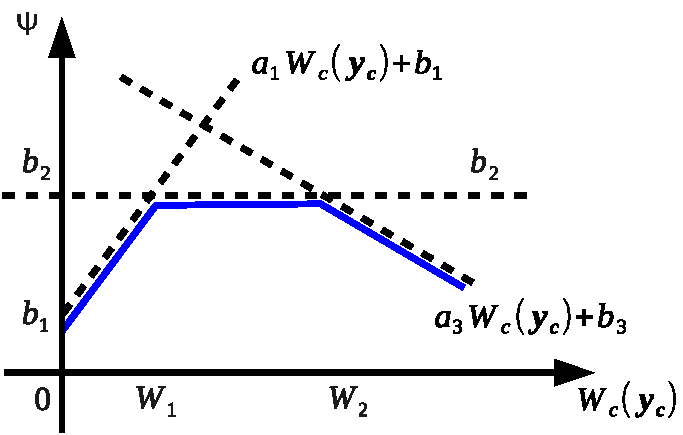
\includegraphics[width=0.6\columnwidth]{Methodology/figures/not_redundant}
  \caption{\label{fig:nonredundant} Example lower linear envelope
    $\psi^H_c\!(\by_c)$ (shown solid) with three terms (dashed).
    When $W_{\!c}(\by_c) \leq W_1$ the first linear function is
    active, when $W_1 < W_{\!c}(\by_c) \leq W_2$ the second
    linear function is active, otherwise the third linear
    function is active.}
\end{figure}

Inference on energy function contains lower linear potentials is
the same as the standard equation~\eqref{eq:energyfunction_UPH}
and is given by:
\begin{align}
  \label{eq:min_energy}
  \by^* = \argmin\energy{\by}
\end{align}

\begin{figure}[ht]
  \centering
  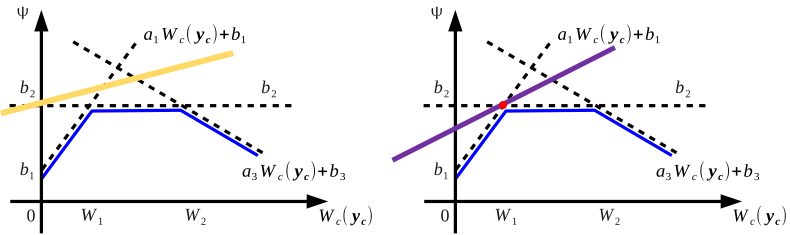
\includegraphics[width=1\columnwidth]{Methodology/figures/redundant}
  \caption{\label{fig:redundant} Example lower linear envelope
    with redundant linear functions. On the left figure, the
    solid yellow line is always inactive. On the right figure,
    the solid purple line intersects $line \; 1$ and $line \; 2$
    at the red point. It's only active when $line \; 1$ and $line
    \; 2$ are both active. Both solid lines are redundant linear
    functions hence can be removed without changing their energy
    function.}
\end{figure}
%
Suppose that parameters $\{(a_k, b_k)\}_{k=1}^K$ are sorted in
decreasing order of $a_k$. From \emph{Definition 3.1}
\cite{gouldlearning} we know that the $k$-th linear function is
said to be \emph{active} if there exists $x \in (0, 1)$ such that
the following two inequalities hold
\begin{align}
  a_{k-1} x + b_{k-1} &> a_k x + b_k \nonumber \\
  a_{k+1} x + b_{k+1} &> a_k x + b_k
  \label{eqn:nonred_in_ab}
\end{align}
%
The $k$-th linear function is said to be \emph{redundant}
(\emph{Definition 3.2}~\cite{gouldlearning}) if it is not active
for any assignment to $\by_c$ in any clique $c \in \C$ or is only
active whenever another linear function is also active.
Figure \ref{fig:redundant} depicts such conditions. As a
result, removing redundant functions from the potential does not
chang the energy function.

To ensure potentials do not contain redundant linear functions,
\citename{gouldlearning} rearranged conditions
\ref{eqn:nonred_in_ab} in terms of $x$ and proposed a condition on
parameters of the envelope. The $k$-th linear function is
not redundant if the following condition is satisfied:
%
\begin{align}
    0
    <
    \frac{b_k - b_{k-1}}{a_{k-1} - a_k}
    <
    \frac{b_{k+1} - b_k}{a_k - a_{k+1}}
    <
    1.
  \label{eq:nonredundant}
\end{align}
%
Another important property of equation~\eqref{eq:min_energy} is
shift invariant~\cite{gouldlearning} (vertically). We write
$\widetilde{\psi}^{H}_c\!(\by_c)$ by shift equation~\eqref{eqn:potential2} vertically
with an abitrary amount $b^{const}\in R$
$$\widetilde{\psi}^{H}_c\!(\by_c) = \min_{k=1, \ldots, K}
\left\{a_k W_{\!c}(\by_c) + b_k + b^\textrm{const} \right\}$$
%
Then we have
\begin{align}
  \argmin_{\by_c} \psi^H_c\!(\by_c)
  = \argmin_{\by_c} \widetilde{\psi}^{H}_c\!(\by_c).
  \label{eq:shift_invariant}
\end{align}
%
Therefore, in the following discussion without loss of generality
we assume $b_1 = 0$ thus $b_k\geq0 \text{\; for \;} k=1,\dots,n$.
%
\subsection{Exact Inference}
\label{sec:exact_inference}

Exact inference on MRFs has been extensively studied in past
years. Researchers found that, energy functions which can be
transformed into quadratic pseudo-Boolean
functions~\cite{Ishikawa:PAMI03,Ishikawa:CVPR09,Rother:CVPR09}
are able to be minimized exactly using \emph{graph-cuts} like
algorithms~\cite{Freedman:CVPR05,Hammer:1965} when they satisfy
submodularity condition~\cite{Boros:MATH02}.
\citename{Kohli:TR08} and \citename{Gould:ICML2011} adapted those
results to perform exact inference on lower linear envelope
potentials. In this section we mainly focus on describing the
\emph{st min cut} graph constructed by
Gould~\cite{Gould:ICML2011,gouldlearning} for exact
inference~\eqref{eq:min_energy} of energy function containing
lower linear envelope potentials.

Following the approach of \citename{Kohli:CVPR10},
\citename{Gould:ICML2011,gouldlearning} transformed the weighted
lower linear envelope potential~\eqref{eqn:potential2} into a
quadratic pseudo-Boolean function by introducing $K-1$ auxiliary
variables $\bz = \left(z_1, \ldots, z_{K-1}\right)$ with $z_k\in
\{0,1\}$:

\begin{align}
  E^c(\by_c, \bz) = a_1 W_{\!c}(\by_c) + b_1
  {}+ \sum_{k = 1}^{K-1} z_k \left( \left(a_{k+1} - a_k\right) W_{\!c}(\by_c) + b_{k+1} - b_k \right)
  \label{eqn:binary_concave_z}
\end{align}

\noindent for a single clique $c \in \C$. Under this formulation,
\citename{Gould:ICML2011,gouldlearning} showed that minimizing
the pseudo-Boolean function over $\bz$ is equivalent to selecting
(one of) the active functions(s) from
equation~\eqref{eqn:potential2}. Another important property of
optimized $\bz$ under this formulation is that it
automatically satisfies the constraint~\cite{gouldlearning}: 

\begin{figure}[t]
  \centering
  \setlength{\tabcolsep}{2pt}
  \begin{tabular}{cc}
    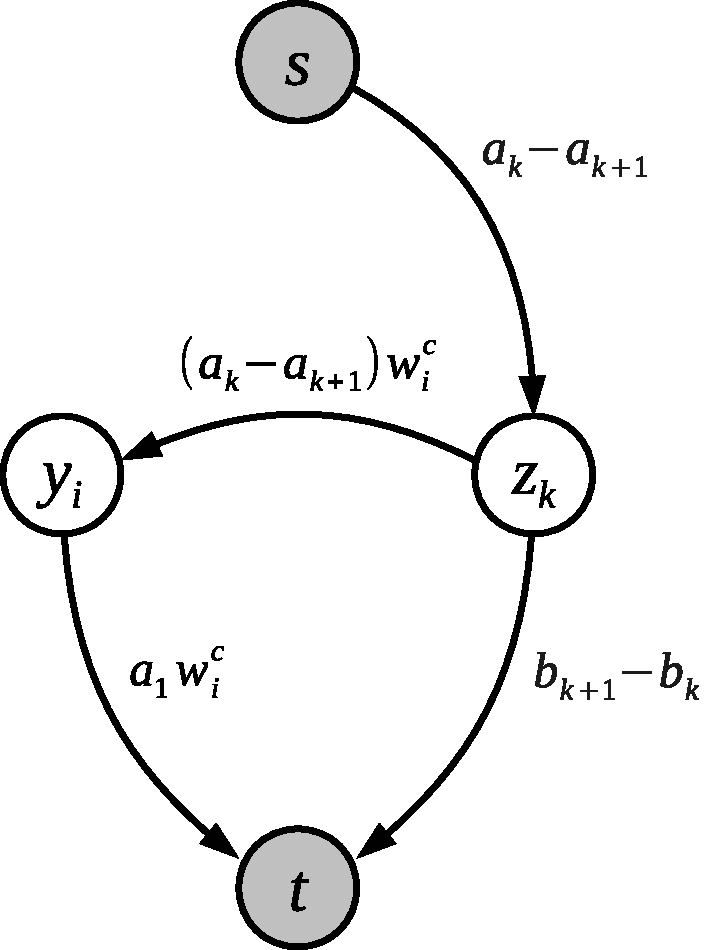
\includegraphics[width=0.45\columnwidth]{Methodology/figures/stmincut}&
                                                                         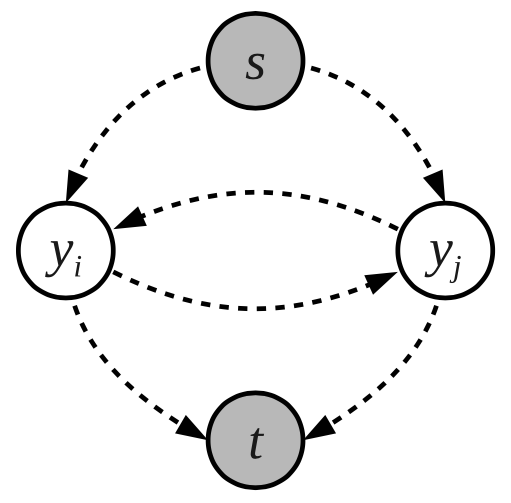
\includegraphics[width=0.5\columnwidth]{Methodology/figures/unary_pairwise.png}\\
                                                                         {\small (a)} & {\small (b)} 
  \end{tabular}
  \caption{\label{fig:stmincut} $st$-graph
    construction~\cite{gouldlearning} for
    equation~\eqref{eqn:posiform}, unary and pairwise terms.
    Every cut corresponds to an assignment to the random
    variables, where variables associated with nodes in the
    ${\cal S}$ set take the value one, and those associated with
    nodes in the $\T$ set take the value zero. With slight abuse
    of notation, we use the variables to denote nodes in our
    graph.}
\end{figure}

\begin{align}
  \label{eq:z_consecutive_constraint}
  z_{k+1} \leq z_k
\end{align}

\noindent this property give rise to further development of
parameter vector~\eqref{eq:llsvm_param} and feature
vector~\eqref{eq:llsvm_feature} which are used in latent
structural SVM.

In order to construct the \emph{st-min-cut} graph,
\citename{gouldlearning} rewrote
equation~\eqref{eqn:binary_concave_z} into
\emph{posiform}~\cite{Boros:MATH02}:

\begin{align}
  \label{eqn:posiform}  
  E^c(\by_c, \bz)
  &= b_1 - (a_1 - a_K) + \sum_{i \in c} a_1 w^c_i y_i
  {}+ \sum_{k = 1}^{K - 1} \left( b_{k+1} - b_k \right) z_k\\
  &+ \sum_{k = 1}^{K - 1} \left( a_k - a_{k+1} \right) \bar{z}_k
  {}+ \sum_{k = 1}^{K - 1} \sum_{i \in c} \left( a_k - a_{k+1}
    \right) w^c_i \bar{y}_i z_k \nonumber
\end{align}

\noindent where $\bar{z}_k = 1 - z_k$ and $\bar{y}_i = 1 - y_i$.
$a_1$ is assumed to be greater than $0$ so that all coefficients
are positive (recall we assume $b_1=0$ in section~\ref{sec:llep}
and we have $a_k > a_{k+1}$ and $b_k < b_{k+1}$). After proving
\emph{submodularity} of the energy function~\eqref{eqn:posiform},
\citename{gouldlearning} constructed the \emph{st-min-cut} graph
based on equation~\eqref{eqn:posiform}.

The construction is explained in \figref{fig:stmincut}. Figure
(a) denotes construction for equation~\eqref{eqn:posiform}. For
each lower linear envelope potential edges are added as follows:
for each $i \in c$, add an edge from $y_i$ to $t$ with weight
$a_1 w^c_i$; for each $i \in c$ and $k = 1, \ldots, K-1$, add an
edge from $z_k$ to $y_i$ with weight $(a_{k} - a_{k+1}) w^c_i$;
and for $k = 1, \ldots, K-1$, add an edge from $s$ to $z_k$ with
weight $a_k - a_{k+1}$ and edge from $z_k$ to $t$ with weight
$b_{k+1} - b_k$. Figure (b) denotes construction for unary and
pairwise terms (see \cite{Kolmogorov:PAMI04}). For unary edges (4
edges on both sides), weights on each edge are corresponding to
values in input unary terms accordingly. For pairwise edges (2
edges in the middle), both edges share the same weight which
equals to the input pairwise term.

\section{Learning the Lower Linear Envelope with Latent Information}
\label{sec:learning}

With the inference algorithm in hand, we now can develop the
learning algorithm for weighted lower linear envelope potentials
using the latent structural SVM framework. We begin by
transforming the equation~\eqref{eqn:binary_concave_z} into a
linear combination of parameter vector and feature vector. Then a
two-step algorithm was developed to solve the latent structural
SVM.


\subsection{Transforming Between Representations}
\label{sec:latent_linEnv_represent}

The latent structural SVM formulation (see
equation~\eqref{eq:latent_ssvm_linearcomb}) requires that the
energy function be expressed as a linear combination of features
and weights while our higher-order potential is represented as
the minimum over a set of linear functions. However,
in~\ref{sec:exact_inference} we reformulated the piesewise linear
functions into a quadratic pseudo-Boolean
function~\eqref{eqn:binary_concave_z} by introducing auxiliary
variables. Now we show function~\eqref{eqn:binary_concave_z}
itself is an inner product of parameter vector and feature vector
with latent information. We first noticed that the function can
be expanded as a summation of $2K-1$ terms:

\begin{align}
  \label{eq:originalenergy}
  E^c(y_c,z)&=a_1W_c(y_c)+b_1+\sum_{k=1}^{K-1}z_k((a_{k+1}-a_k)W_c(y_c)+b_{k+1}-b_k)\nonumber\\ 
            &=a_1W_c(y_c)+\sum_{k=1}^{K-1}(a_{k+1}-a_k)z_kW_c(y_c)+\sum_{k=1}^{K-1}(b_{k+1}-b_k)z_k
\end{align}

Here we use the fact of equation~\eqref{eq:shift_invariant} and
let $b_1=0$. Now we can reparameterize the energy function
as
\begin{align}
  \label{eq:llsvm_innerprod_energy}
  E^c(\by_c,\bz; \btheta) = \btheta^T \! \phi(\by_c,\bz)
\end{align}

\noindent where:

\begin{equation}
\label{eq:llsvm_param}
  \theta_k = \left\{
    \begin{aligned}
      & a_1	& \text{for} \ k=1\\
      & a_k-a_{k-1} & \text{for}\ 1< k \leq K\\
      & b_{k+1-K}-b_{k-K} & \text{for} \ K<k\le2K-1\\
    \end{aligned}
  \right.
\end{equation}

\begin{equation}
\label{eq:llsvm_feature}
  \phi_k = \left\{
		\begin{aligned}
      & W_c(\by_c) 	& \text{for} \ k=1\\
      & W_c(\by_c)\bz_k & \text{for}\ 1<k\le K\\
      & \bz_k & \text{for} \ K<k\le2K-1\\
		\end{aligned}
  \right.
\end{equation}

Under this formulation, inference
problems~\eqref{eq:latentssvm_full_inf}
and~\eqref{eq:latentssvm_latent_inf} introduced in
section~\ref{sec:latent-struct-svms} can be written as:

\begin{align}
  \label{eq:linenv_full_inf}
  (\mathbf{\hat{y}}_k(\btheta),\mathbf{\hat{z}}_k(\theta))=\argmin_{(\mathbf{y}
  \times \mathbf{z}) \in \mathcal{Y} \times \mathcal{Z}}
  \btheta^T\cdot\phi(\mathbf{y}_k,\mathbf{z}_k)
\end{align}
and
\begin{align}
  \label{eq:linenv_latent_inf}
  \mathbf{z}^*_k(\btheta) = \argmin_{\mathbf{z} \in \mathcal{Z}}
  \btheta^T \cdot \phi(\mathbf{y}_k,\mathbf{z}_k)
\end{align}

There are 2 facts worth to mention. The first fact is
that in our previous construction of minimum-$st$-cut graph the
latent variable $\bz$ is already included. Therefore, we can
apply our inference algorithm directly on our 2 new formulations.

However, for equation~\eqref{eq:linenv_latent_inf} there exists
more efficient algorithm. At training stage the ground-truth
labels $y_i$ is a function input thus completely observed.
Therefore, the term $((a_{k+1}-a_k)W_c(\by_c)+b_{k+1}-b_k)$ in
equation~\ref{eq:originalenergy} becomes constant. So we can
infer latent variable $\bz$ explicitly by:
\begin{align}
  \label{eq:linenv_effi_infer_latent}
  z_k^c &=
          \begin{cases}
            0 & \text{if $((a_{k+1}-a_k)W_c(y_c)+b_{k+1}-b_k)\geq0$} \\
            1 & \text{otherwise}.
          \end{cases}
\end{align}

\begin{figure}[t]
  \centering
  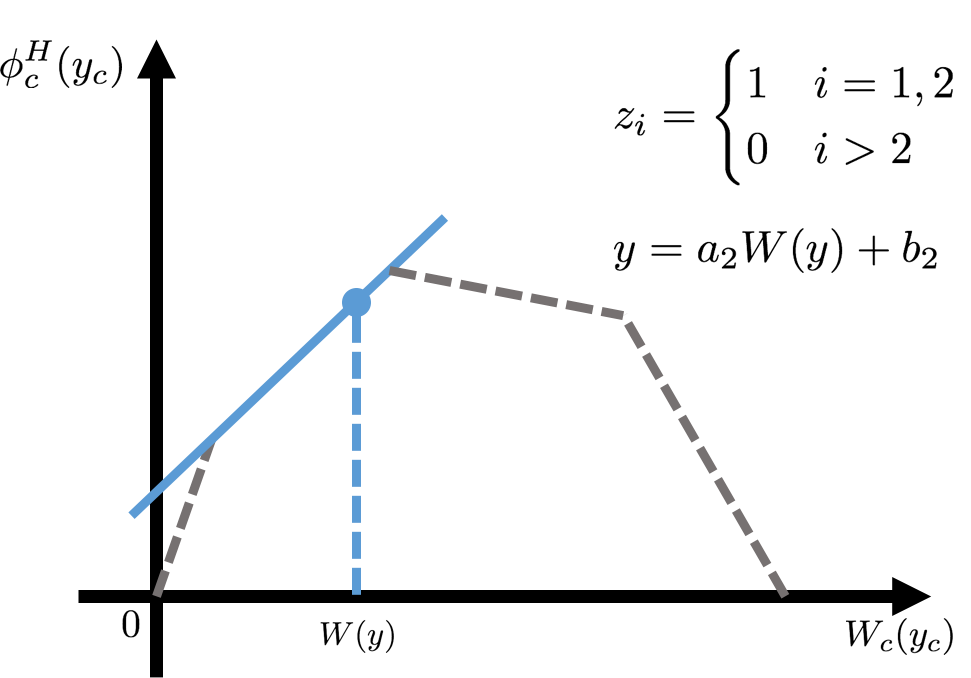
\includegraphics[width=0.8\columnwidth]{Methodology/figures/linEnvLatentFig.png}
  \caption{\label{fig:concave} Example piecewise-linear concave
    function of $W_{\!c}(\by_c) = \sum_{i \in c} w^c_i y_i$.
    Assume the second linear function is active namely
    $\bz^c=(1,1,0,0)$. The result of linear combination of
    parameter vector and feature vector is same as quadratic
    psuedo-Boolean function.}
\end{figure}

To show the equivalence between
equation~\eqref{eqn:binary_concave_z} and
equation~\eqref{eq:llsvm_innerprod_energy} we consider the
example illustrated in figure~\ref{fig:concave}. Assume the
inferred latent vector $\bz^c=(1,1,0,0)$. Plug it into
equation~\eqref{eq:llsvm_feature} the energy function can be
written as:
\begin{align*}
  E^c(\by_c,\bz; \btheta) &=
  \begin{bmatrix}
    a_1\\
    a_2-a_1\\
    a_3-a_2\\
    a_4-a_3\\
    b_2\\
    b_3-b_2\\
    b_4-b_3
  \end{bmatrix}^T
  \begin{bmatrix}
    W_c(\by_c) \\
    W_c(\by_c) \\
    0\\
    0\\
    1\\
    0\\
    0
  \end{bmatrix}\\
  &=a_1W_c(\by_c)+(a_2-a_1)W_c(\by_c)+b_2\\
  &=a_2W_c(\by_c)+b_2
\end{align*}

Therefore, assignments inferred by graph-cut algorithm can be
directly encoded into a linear combination by using our latent
structural SVM formulation for learning purpose. The remaining
task is to ensure the concavity of $\btheta$. We do this by
adding the following constraint:

\begin{align}
  A\btheta\geq0 \text{,\;~~~} A=
                  \begin{bmatrix}
                    1 & \mathbf{0} & \mathbf{0}\\
                    \mathbf{0} & -\mathbf{1} & \mathbf{0}\\
                    \mathbf{0} & \mathbf{0} & \mathbf{P}
                  \end{bmatrix}\in \mathbb{R}^{(2K-1)\times(2K-1)}
\end{align}

\noindent where $-\mathbf{1}$ is a matrix of size $(K-1)\times(K-1)$ and
$\mathbf{P}$ is an identity matrix of size $(K-1)\times(K-1)$.

One subtle problem we found during experiments is that the
algorithm can be stuck small numerical value. To avoid this we
add small slack variables $\epsilon$ on those constraints:

\begin{align}
  \label{eq:concave_constraint}
  A\btheta\geq\epsilon \text{,\;~~~} A=
                  \begin{bmatrix}
                    1 & \mathbf{0} & \mathbf{0}\\
                    \mathbf{0} & -\mathbf{1} & \mathbf{0}\\
                    \mathbf{0} & \mathbf{0} & \mathbf{P}
                  \end{bmatrix}\in \mathbb{R}^{(2K-1)\times(2K-1)}
\end{align}

\noindent where $\epsilon$ usually equal to $\mathbf{1}^{-15}$ in our
experiments.

\subsection{Latent Structural SVM Learning}
\label{sec:mrflssvm_learning_algo}

With the inner product formulation
(equation~\eqref{eq:llsvm_innerprod_energy}) of higher order
energy function in hand, we now able to develop our latent
structural SVM learning algorithm. The energy function (higher
order function together with unary and pairwise functions) can be
written as:
\begin{equation}
  E_{all}(y,z) = \begin{bmatrix}
    \btheta^H\\
    \theta^{unary}\\
    \theta^{pairwise}
  \end{bmatrix}^T 
  \cdot \begin{bmatrix}
    \phi^H\\
    \phi^{unary}\\
    \phi^{pairwise}
  \end{bmatrix}=\theta_{all}^T\cdot\phi_{all}
\end{equation}
where $\btheta^H\in \real$ is the parameter vector in higher
order equation~\eqref{eq:llsvm_innerprod_energy} of size $2K-1$.
$\theta^{unary}$ and $\theta^{pairwise}$ are both scalars.
$\phi^\textrm{unary} = \sum_i \psi^U_i\!(y_i)$ and
$\phi^\textrm{pairwise} = \sum_{ij} \psi^P_{ij}(y_i, y_j)$.
Therefore, the size of $\theta_{all}$ is $2K+1$.

Plug equation~\eqref{eq:linenv_full_inf} and
equation~\eqref{eq:linenv_latent_inf} into object
function~\eqref{eq:latent_ssvm_object}, the latent structural SVM
object function for our problem can be derived as a difference of
two convex functions:

\begin{align}
\label{eq:lssvm_object}
  \min_\theta\bigg(\frac{1}{2}\|\theta\|^2+
  C\sum_{i=1}^{n}\big(\max_{(\mathbf{\hat{y}} \times
  \mathbf{\hat{z}}) \in \mathcal{Y} \times \mathcal{Z}}
  [\theta\cdot\phi(\mathbf{\hat{y}},\mathbf{\hat{z}}) +
  \Delta(\mathbf{y}_i,\mathbf{\hat{y}},\mathbf{\hat{z}})]\big)\bigg)\\
  -C\sum_{i=1}^{n}\big(\max_{\mathbf{z} \in \mathcal{Z}} \theta \cdot
  \phi(\mathbf{y}_i,\mathbf{z})\big)\nonumber
\end{align}

As mentioned by \citename{yu2009learning} the Concave-Convex
Procedure (CCCP)~\cite{yuille2002concave} can be used to solve the
optimization problem. Our algorithm contains two stages. We first
imputes the latent variables $\bz$ explicitly by
equation~\eqref{eq:linenv_latent_inf}. Namely solving the
``latent variable completion'' problem~\cite{yu2009learning}:

\begin{align}
  \bz_i^*=\argmax_{\mathbf{z} \in \mathcal{Z}} \theta \cdot
  \phi(\mathbf{y}_i,\mathbf{z})
\end{align}

The inference result $z_i^*$ for $i=1,\dots,n$ is used as
completely observed for later stage. With the latent variable
$z_i^*$ which best explains the ground-truth data $y_i$ in hand,
updating the parameter vector $\btheta$ is similar to solve the
standard max-margin optimization problem described
in~\cite{gouldlearning}:

\begin{align}
\label{eq:mrflssvm_object}
  \min_\theta\bigg(\frac{1}{2}\|\theta\|^2+
  C\sum_{i=1}^{n}\big(\max_{(\mathbf{\hat{y}} \times
  \mathbf{\hat{z}}) \in \mathcal{Y} \times \mathcal{Z}}
  [\theta\cdot\phi(\mathbf{\hat{y}},\mathbf{\hat{z}}) +
  \Delta(\mathbf{y}_i,\mathbf{\hat{y}},\mathbf{\hat{z}})]\big)\bigg)\\
  -C\sum_{i=1}^{n}\big(\theta \cdot
  \phi(\mathbf{y}_i,\mathbf{z}_i^*)\big) \nonumber
\end{align}

The last problem remaining is the initialization method. Because
our objective function~\eqref{eq:mrflssvm_object} is not convex
and the CCCP algorithm is only guaranteed to converge to a local
minimum or saddle point\cite{yuille2002concave}, initialization
of $\btheta$ might affect the performance of our algorithm. Since
there are no theoretical solution for this problem, we only
propose an empirical \algref{alg:init_theta}:

\begin{algorithm}[ht]
  \begin{algorithmic}[1]
    \STATE{$gap=\frac{1}{K}$, $a_1=\U(0,1e6)$, $b_1=0$,
      $sp_1=(0,0)$, $w_0=0$, $counter=2$} \FOR{each
      clique $c\in \C$} \STATE{Compute weighted clique value
      $w_c=W_c(y_C)$} \IF{$w_c-w_{c-1}>gap$}
    \STATE{$upbound = a_{counter}w_c+b_{counter}$\\
      $sp_{counter}=(w_c,\U(upbound-0.5,upbound))$\\
      Calculate $a_{counter}$ and $b_{counter}$ using
      $sp_{counter-1}$ and $sp_{counter}$\\
      $counter=counter+1$}
    \ENDIF
    \ENDFOR
    \STATE{If $counter<K$, remaining $a$s and $b$s are all set to
      be $a_{counter}$ and $b_{counter}$} \STATE{Calculate
      $\btheta$ using $\{a_k,b_k\}_{k=1}^K$}
  \end{algorithmic}
  \caption{\label{alg:init_theta} Empirical initialization
    algorithm for $\btheta$}
\end{algorithm}

We assume that the more evenly distributed of $W_c(Y_c)$ where
$c\in\C$ on $x$ axis, the more rich representation (number of
linear functions) the energy function should have. In order to
initialize $\btheta$, we first determine the x-coordinate of
sampled points $sp$. Then we sample its y-coordinate from a
uniform distribution $\U(upbound,upbound-0.5)$ to add some
randomness in our initialization as well as maintain concavity.
Linear parameters $a_k$ and $b_k$ are later calculated using
those sampled points $sp_k$ and $sp_{k-1}$. At last we encode
$\{a_k,b_k\}_{k=1}^K$ into $\btheta$ using
equation~\eqref{eq:llsvm_param}.

Our optimization algorithm is summarized in
\algref{alg:learning}.

\begin{algorithm}[hb]
  \begin{algorithmic}[1]
    \STATE{Set $MaxIter = 100$}
    \STATE{ {\bf input} training set $\{\by_i\}_{i=1}^{n}$, regularization constant $C > 0$,
      and tolerance $\epsilon \geq 0$}
    \STATE{Initialize $\btheta$ using \algref{alg:init_theta}}
    \REPEAT
    \STATE{Set $iter = 0$}
    \FOR{each training example, $i = 1, \ldots, n$}
    \STATE{compute $ \bz_i^*=\argmax_{\mathbf{z} \in \mathcal{Z}}
      \theta \cdot \phi(\mathbf{y}_i,\mathbf{z}) $}
    \ENDFOR

    \STATE{ {\bf initialize} active constraints set $\C_i = \{ \}$ for all $i$}
    \REPEAT

    \STATE{solve the quadratic programming problem in
      equation~\ref{eq:mrflssvm_object} with respect to active
      constraints set $\C_i$ for all $i$ and concavity constraints
      $A\btheta\geq \epsilon$ to get
      $\hat{\btheta}$ and $\hat{\bxi}$}

    \FOR{each training example, $i = 1, \ldots, n$}
    \STATE{compute $\hat{\by_i},\hat{\bz_i} = \argmin_{\by}
      E(\by,\bz; \hat{\btheta}) - \Delta(\by, \bz, \by_i)$}
    \IF{$\hat{\xi}_i + \epsilon \!<\! \Delta(\hat{\by_i},
      \hat{\bz_i}, \by_i) -
      E(\hat{\by_i},\hat{\bz_i}; \hat{\btheta}) + E(\by_i, \bz_i^*; \hat{\btheta})$}
    \STATE{$\C_i \leftarrow \C_i \cup \{\by_i^\star\}$}
    \ENDIF
    \ENDFOR
    \UNTIL{no more violated constraints}
    \STATE{ {\bf return} parameters $\hat{\btheta}$}
    \STATE{Set $iter = iter+1$}

    \UNTIL{$iter\geq MaxIter$}
    \STATE{ {\bf return} parameters $\hat{\btheta}$}
  \end{algorithmic}
  \caption{\label{alg:learning} Learning lower linear envelope
    MRFs with latent variables.}
\end{algorithm}



\clearpage
\cleardoublepage


%%% Local Variables:
%%% mode: latex
%%% TeX-master: "../thesis"
%%% End:

%%
%% Template Experiments.tex
%%

\chapter{Experiments}
\label{cha:Experiments}

In this chapter, we follow our previous approach
in~\cite{gouldlearning} and conduct two experiments with
different purposes. We first examine our method's effectiveness
by comparing our results with~\cite{gouldlearning,Gould:ICML2011}
on a synthetic checkerboard. We then extend our work to the
real-world ``GrabCut'' problem introduced in
section~\ref{sec:grabcut} and comparing our result with previous
researches \cite{Rother:SIGGRAPH04} to investigate
our new methods' performance.

\section{Synthetic Checkerboard}
\label{sec:synth-check}

Since the main contribution of our work is extending our previous
approximate formulation of lower linear envelope potentials to an
exactly formulation, it is necessary to compare the results on
synthetic checkerboard to previous work~\cite{gouldlearning}.

In this section we will experiment our method on three different
problem instances: checkerboard with squares containing
monotonous color~\ref{sec:monot-color-squar}, checkerboard with
squares containing more pixels of one color over
another~\ref{sec:unbal-color-squar} and checkerboard with
uniformly colored squares containing unbalanced
color~\ref{sec:unif-distr-squar}.

\subsection{Experiment Settings}
\label{sec:experiment-settings}

An image of synthetic checkerboard contains $8 \times 8$ pixel
squares. Each square (clique) contains $16 \times 16$ (256)
pixels. The color of each pixel is either black $0$ or white $1$.
Given a ground-truth checkerboard image
$\by^*=y^*_1,\dots,y^*_{16384}$, the observed unary terms
$\by=y_1,\dots,y_{16384}$ are generated as followings. Let
$\eta_0$ and $\eta_1$ be the signal-to-noise ratios for the black
and white squares, the unary terms are generated by destroying
groud-truth label to noisy input
\begin{align}
  \label{eq:noisy_checkerboard}
  y_i = \eta_0 \ind{y^\star_i = 0} - \eta_1 \ind{y^\star_i = 1} + \delta_i
\end{align}
where $\delta_i
\sim \U(-1, 1)$ is additive i.i.d.\ uniform noise. $\ind{x}$ is
an indicator function which equals $1$ when $x$ is true and $0$
otherwise. The task is to recover the ground-truth checkerboard
from the noisy input.

Our MRF is constructed on this image by associating each node in
the MRF to each pixel in the image. Thus our MRF contains $8
\times 8 \times 256 = 16,384$ variables. The energy function used
in this experiment follows equation~\eqref{eq:energyfunction_UPH}
without pairwise terms.

\begin{align}
  \label{eq:syncheck_energy}
  E(\by;\btheta)=\theta^U\sum_{i\in \N}{\phi^U(\by_i)}+
  \sum_{\by_c\in \C}{\phi^H(\by_c,\bz_c;\btheta^H)}
\end{align}
where $\phi^U(\by_i)=\by_i$ and $\theta^U$ is a scalar weight for
unary terms. $\phi^H(\by_c,\bz_c;\btheta^H)=\btheta^{H\;T} \!
\phi(\by_c,\bz_c)$ is equivalent to
equation~\eqref{eq:llsvm_innerprod_energy} and added for each
square (clique $c$) in the checkerboard. The number of linear
equations $K$ in equation~\eqref{eq:llsvm_param} is set to be
$10$. The parameters $\theta^U$ and $\btheta^H$ are learned using
\algref{alg:learning} with $MaxIter=100$. 

\subsection{Monotonous Colored Squares}
\label{sec:monot-color-squar}

\begin{figure}[hb]
  \centering
  \setlength{\tabcolsep}{2pt}
  \begin{tabular}{cc}
    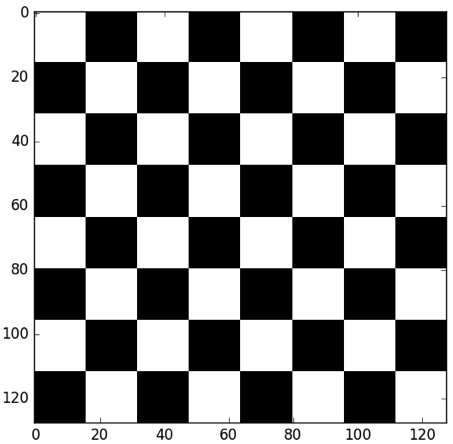
\includegraphics[width=0.5\columnwidth]{Experiments/figures/mono_gt.png}&
                                                                            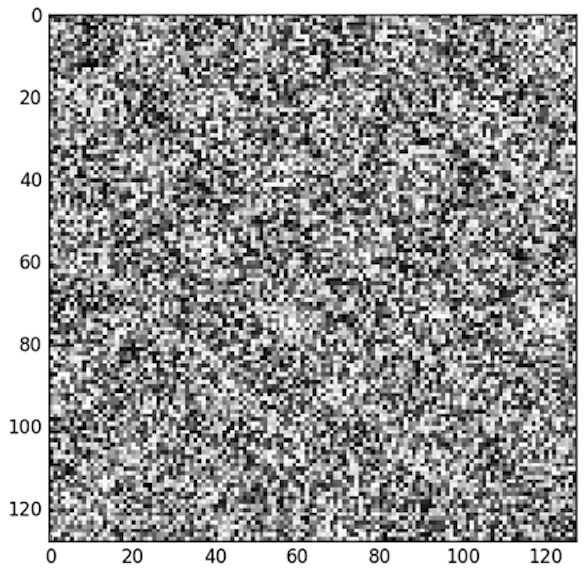
\includegraphics[width=0.5\columnwidth]{Experiments/figures/mono_noisy.png}\\
    {\small (a)} & {\small (b)} 
  \end{tabular}
  \caption{\label{fig:mono_checkerboard} Example for monotonous
    colored squares. figure (a) is the ground-truth checkerboard.
    Figure (b) is the noisy input (unary terms) destroyed by
    equation~\eqref{eq:noisy_checkerboard}}
\end{figure}

We first repeat our previous black and white checkerboard
experiment~\cite{Gould:ICML2011,gouldlearning} in order to
examine the correctness of our new formulation. Each clique
(square) $c\in \C$ in the checkerboard contains either all white
pixels $y_i=1 ,\;\forall i \in c$ or all black pixels $y_i=0
,\;\forall i \in c$. Figure~\ref{fig:mono_checkerboard}
illustrates the ground-truth checkerboard and the noisy input
destroyed by equation~\eqref{eq:noisy_checkerboard} with
$\eta_0=\eta_1=0.1$. Figure~\ref{fig:mono_results} shows the
results of our new method (on the bottom) together with our
previous method~\cite{gouldlearning} (on the top).

\begin{figure}[ht]
  \centering
  \setlength{\tabcolsep}{2pt}
  \begin{tabular}{cc}
    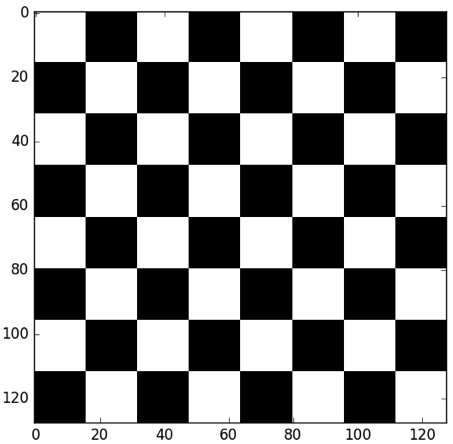
\includegraphics[width=0.3\columnwidth]{Experiments/figures/mono_gt.png}&
                                                                              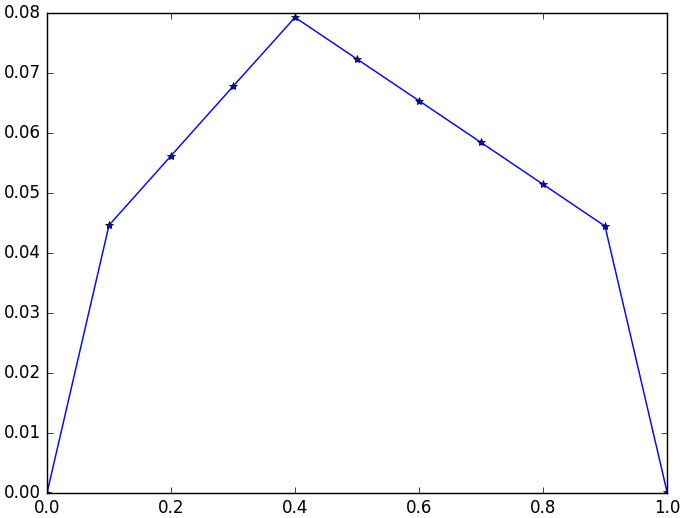
\includegraphics[width=0.4\columnwidth]{Experiments/figures/mono_old.png}\\
    {\small (a)} & {\small (b)} \\
    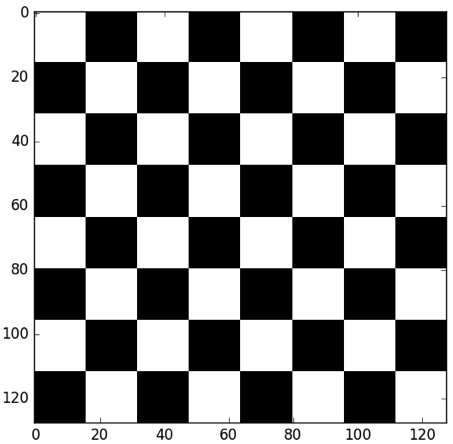
\includegraphics[width=0.3\columnwidth]{Experiments/figures/mono_gt.png}&
                                                                              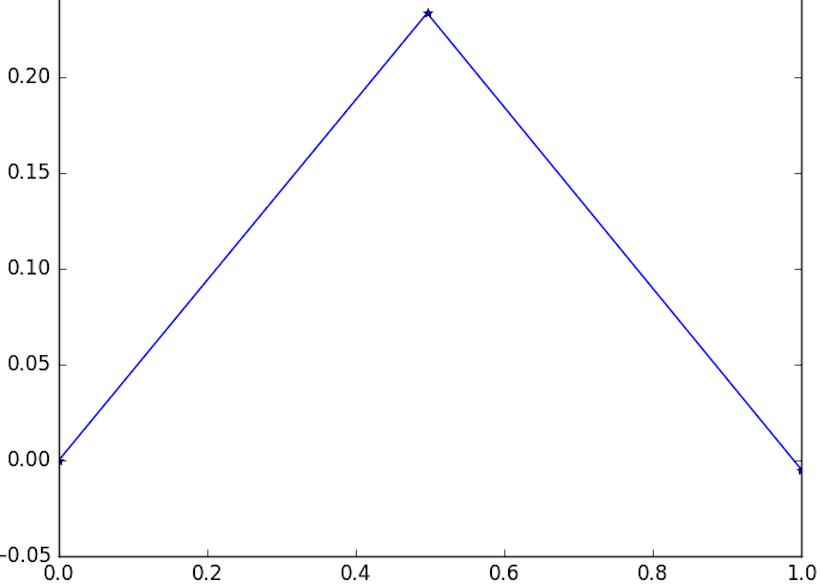
\includegraphics[width=0.4\columnwidth]{Experiments/figures/mono_new.png}\\
    {\small (c)} & {\small (d)} 
  \end{tabular}
  \caption{\label{fig:mono_results} Results comparison for
    monotonous colored squares. Figure (a) and Figure (c) are
    inferred checkerboard from our previous and current
    formulation separately. Figure (b) and Figure (d) are lower
    linear envelopes learned by each formulation.}
\end{figure}

From figure~\ref{fig:mono_results} we conclude that both
formulations can recover checkerboard perfectly so our new
formulation's accuracy is as good as previous one. However,
there are significant differences between structural SVM
formulation (previous method) and latent structural SVM
formulation. There are $10$ active linear functions in
figure~\ref{fig:mono_results} (b) while there are only $2$ active
linear functions in figure~\ref{fig:mono_results} (d). Shapes
learned by each formulation are also significantly different.

In general, the second result is more preferable than the first
one. The reason is despite the image contains 64 cliques, there
are only two kinds of squares in the image: completely black and
completely white. Accordingly, our model only see two kinds of
cliques: completely $0$s (black) and completely $1$s (white). In
this case, a lower linear envelope contains two linear functions
is enough for encoding consistency information. This is reflected
in figure~\ref{fig:mono_results} (d) which gives least penalty
(0) when the clique value $W_C(y_c)$ equals either $0$ or $1$. It
gives the highest penalty when $W_C(y_c)$ is in the middle
because our model has least probability seen that in training
data. The results certificates that our latent structural SVM
formulation can learn lower linear envelope exactly. Therefore,
we say that our new method learns more preferable lower linear
envelope.

In terms of computational performance, because our initial point
are generated randomly using \algref{alg:init_theta}, the
performance various between runnings. On average it takes 2
\emph{outer loops} and 47 \emph{inner loops} to converge. Which
means the latent structural SVM formulation spends $3.5$ times
iterations to converge than previous one ($27$ iterations).
Each \emph{inner loop} took under 1s with inference taking about
120ms on a $2.7$GHz dual-core Intel CPU, which is the same as our
previous method.



\subsection{Unbalanced Colored Squares}
\label{sec:unbal-color-squar}

Experiment in section~\ref{sec:monot-color-squar} proves that our
latent structural SVM formulation can learn the lower linear
envelope exactly. In this section we conduct further experiment
to investigate its capability of representing unbalanced input.
The desirable result of this experiment should be the shape of
the lower linear envelope shifting along with the changing of
input data.

We design our checkerboards contain unbalanced colored squares as
shown in figure~\ref{fig:unba_checkerboard}.

\begin{figure}[hb]
  \centering
  \setlength{\tabcolsep}{2pt}
  \begin{tabular}{cc}
    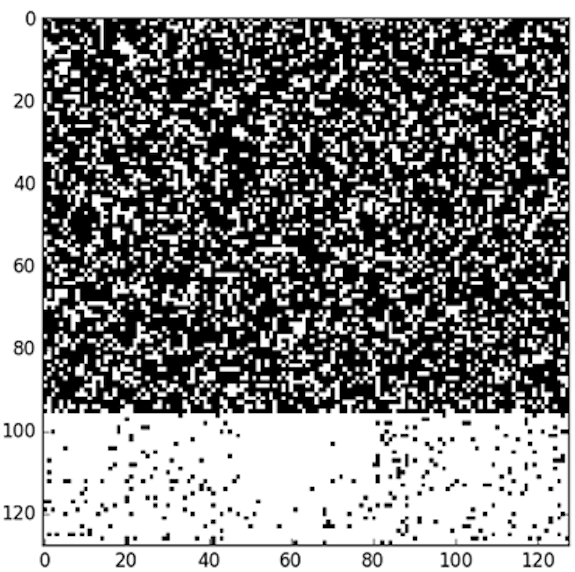
\includegraphics[width=0.5\columnwidth]{Experiments/figures/unba_black.png}&
                                                                            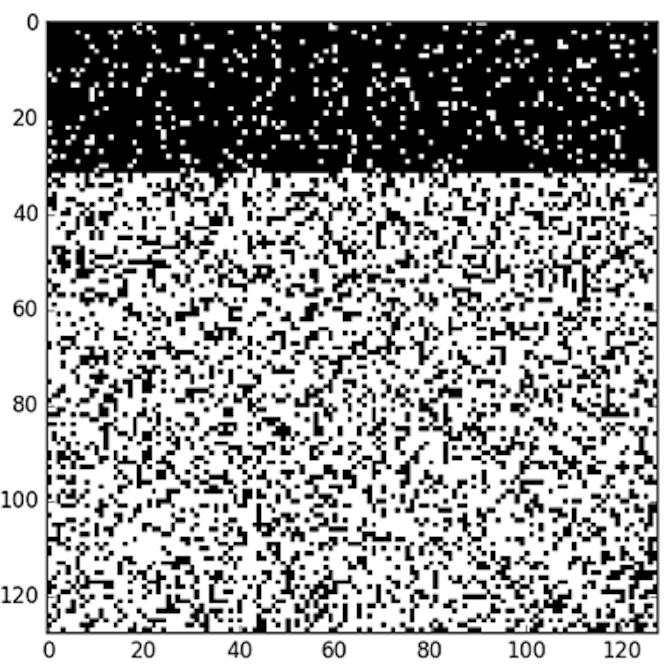
\includegraphics[width=0.5\columnwidth]{Experiments/figures/unba_white.png}\\
    {\small (a)} & {\small (b)} 
  \end{tabular}
  \caption{\label{fig:unba_checkerboard} Example for unbalanced
    colored squares. In figure (a) $75\%$ cliques contain more
    than $85\%$ black pixels while $25\%$ cliques contain more
    than $85\%$ white pixels. Figure (b) is the opposite of
    figure (a)}
\end{figure}

As before, figure~\ref{fig:unba_results} shows results learned by
structural SVM (top row) and latent structural SVM (bottom row).
The accuracy performance of both methods are almost the same.
Both methods are able to recover $45\%-50\%$ pixels. The shape of
each formulations' results are both preferable and very similar
when compared to each other. The most significant difference is
the number of linear functions (10 active linear functions v.s.
2). In terms of computational performance, our previous method
only takes $10$ iterations to converge while the latent
structural SVM formulation takes $89$ iterations. Our new method
is much more computational expensive than our previous method.

\begin{figure}[ht]
  \centering
  \setlength{\tabcolsep}{2pt}
  \begin{tabular}{cc}
    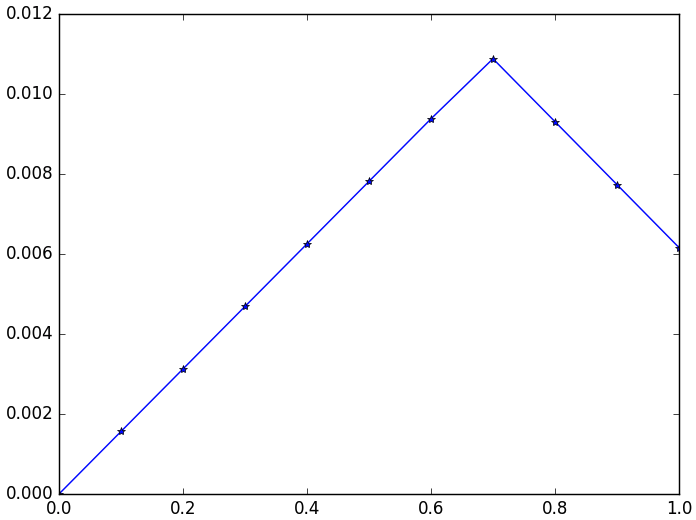
\includegraphics[width=0.5\columnwidth]{Experiments/figures/unba_black_res_old.png}&
                                                                              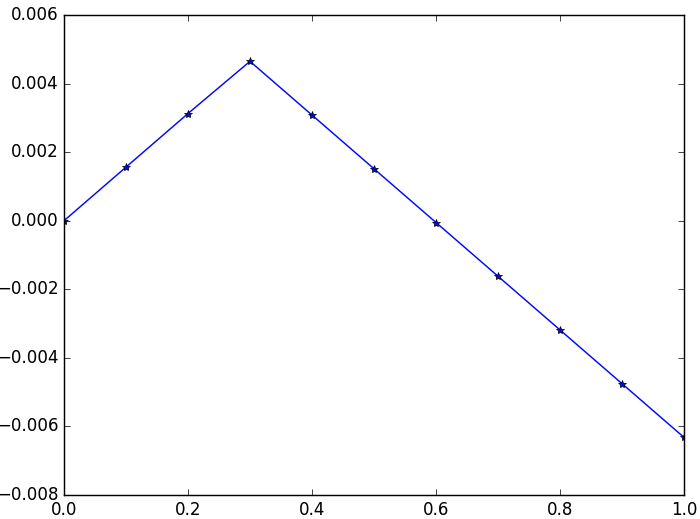
\includegraphics[width=0.5\columnwidth]{Experiments/figures/unba_white_res_old.png}\\
    {\small (a)} & {\small (b)} \\
    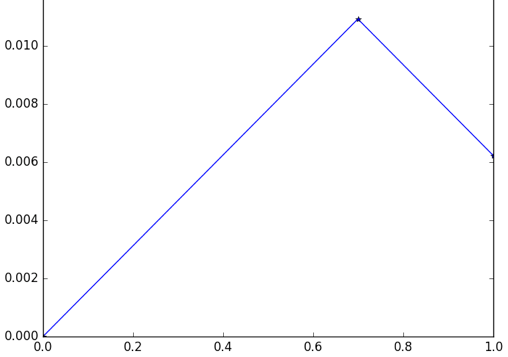
\includegraphics[width=0.5\columnwidth]{Experiments/figures/unba_black_res_new.png}&
                                                                              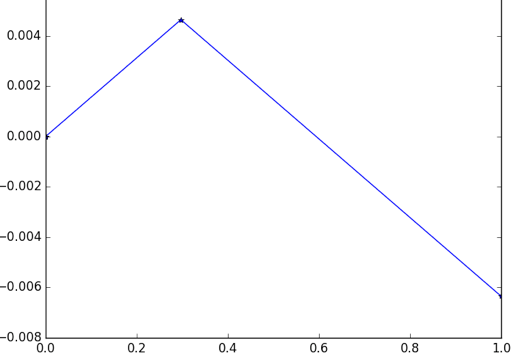
\includegraphics[width=0.5\columnwidth]{Experiments/figures/unba_white_res_new.png}\\
    {\small (c)} & {\small (d)} 
  \end{tabular}
  \caption{\label{fig:unba_results} Results comparison for
    unbalanced colored squares. Figure (a) and Figure (b) are
    lower linear (more black and more white) envelopes learned by
    structural SVM. Figure (c) and Figure (d) are learned by
    latent structural SVM.}
\end{figure}

\bigskip
\bigskip
\bigskip
\bigskip
\bigskip
\bigskip

\subsection{Uniformly Colored Squares}
\label{sec:unif-distr-squar}

All of the above experiments show that our new method can
significantly simplify the shape of the lower linear envelope
function while maintaining the inference performance at the same
level. However, one significant cost is the computational
performance. It still remains obscure if there exists any other
advantages. In this section we design a much harder problem.
$W_c(y_c)$ is uniformly distributed from $0$ to $1$.
Figure~\ref{fig:ba_gt} shows the result. The preferable shape of
the lower linear envelope should contain a line which is parallel
to the x-axis.

\begin{figure}[t]
  \centering
  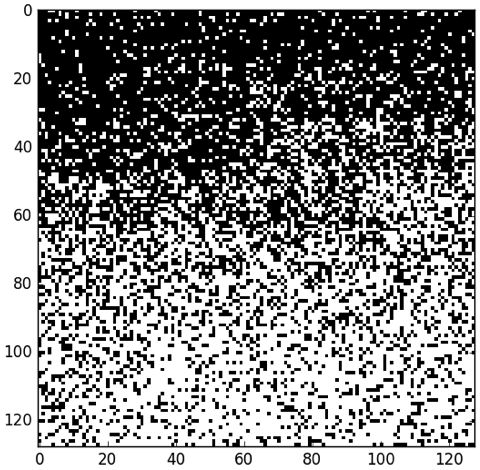
\includegraphics[width=0.5\columnwidth]{Experiments/figures/ba_gt.png}
  \caption{\label{fig:ba_gt} Uniformly colored squares example.
    $W_{\!c}(\by_c) = \sum_{i \in c} w^c_i y_i$ is uniformly
    distributed from $0$ to $1$.}
\end{figure}

Results are shown in figure~\ref{fig:ba_res}. As we can see
that shapes are very different between two formulations. Our
latent structural formulation (figure~\ref{fig:ba_res} (b))
learned a very flat representation of the lower linear envelope
function, which is much preferable, while the structural SVM
formulation preserves much concavity in the shape. This might
because in previous work~\cite{gouldlearning,Gould:ICML2011}
we imposed strict concave constraints on parameter vector
$\btheta$.

The performance of accuracy also various significantly. Under
this formulation our new method is still able to recover
$45\%-50\%$ pixels while our previous can only recover
$25\%-30\%$ pixels on average. Therefore, our new formulation
finally outperforms previous one. In terms of computational
performance, the new formulation takes $129$ \emph{inner loops}
in total (2 \emph{outer loops}) while our previous formulation
takes $75$ iterations to converge. Although the new formulation
is still more computational expensive than previous one, the gap
decreases significantly.

We consider all of those improvements are due to our new method
is able to learn the lower linear envelope exactly.

One subtle thing is that the linear function on the right side in
figure~\ref{fig:ba_res} (b) decreases sharply which seems
abnormally at first glance. The reason is that we assume $b_1=0$
in section~\ref{sec:llep} which fixes the y-intercept of the
first linear function to be zero. Therefore the last linear
function can be arbitrarily deep while the first linear function
is fixed at the original point.

\clearpage

\begin{figure}[ht]
  \centering
  \setlength{\tabcolsep}{2pt}
  \begin{tabular}{cc}
    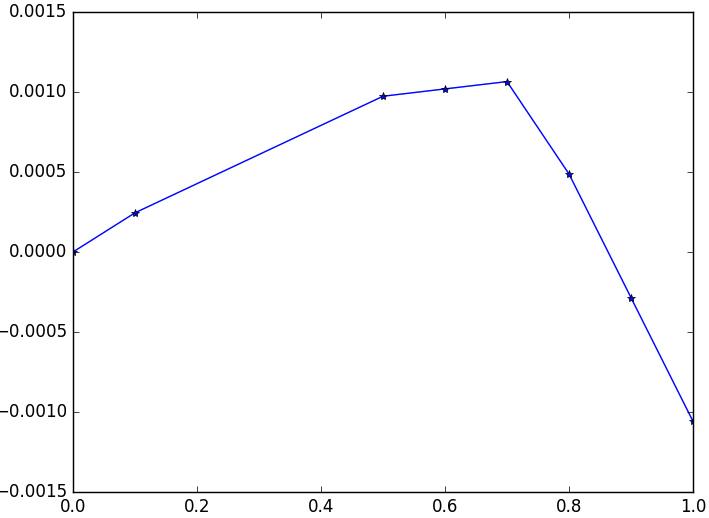
\includegraphics[width=0.5\columnwidth]{Experiments/figures/ba_res_old.png}&
                                                                            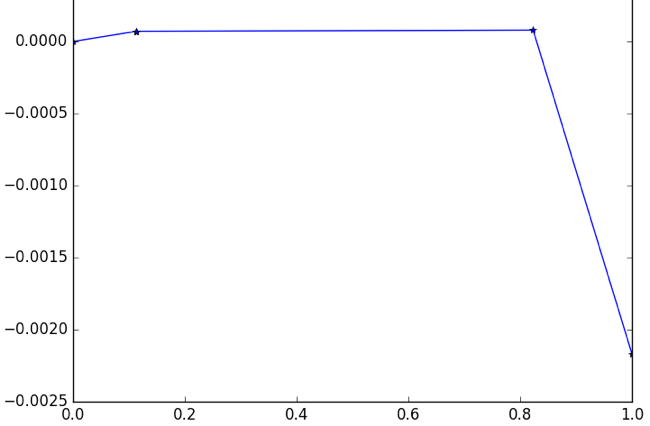
\includegraphics[width=0.55\columnwidth]{Experiments/figures/ba_res_new.png}\\
    {\small (a)} & {\small (b)} 
  \end{tabular}
  \caption{\label{fig:ba_res} Results of uniformly colored
    squares experiment. Figure (a) is the result learned by
    structural SVM formulation. Figure (b) is the result learned
    by latent structural SVM formulation.}
\end{figure}

\subsection{Conclusions}
\label{sec:synth-check-conc}

From above experiments we conclude our findings as followings:

\begin{itemize}
\item All of those experiments verified that our latent
  structural formulation is able learn the lower linear envelope
  exactly.
\item In general (see section~\ref{sec:monot-color-squar} and
  section~\ref{sec:unbal-color-squar}), our new method have
  equivalent accuracy performance to our old method (structural
  SVM formulation\cite{Gould:ICML2011,gouldlearning}).
\item In terms of computational performance, the new formulation
  is much more computational expensive than the previous one
  during training. However, it is more efficient during testing
  due to it simplicity for the lower linear envelope potentials.
\item For harder problem (see
  section~\ref{sec:unif-distr-squar}), the new method outperforms
  the previous one significantly. The gap of computational
  performance also decreases a significant amount.
\end{itemize}

\clearpage

\section{Foreground Extraction}
\label{sec:foregr-extr}

To evaluate our method on real-world applications, we repeat the
``Interactive Figure-Ground Segmentation'' experiment in our
previous researches~\cite{gouldlearning,Gould:ICML2011}. As
described in section~\ref{sec:grabcut}, the goal of this
experiment is to extract foreground pixels from a bounding box of
the object. We follow settings in previous work and replace
the max margin algorithm with latent structural SVM
\algref{alg:learning}.

\subsection{Experiment Settings}
\label{sec:experiment-settings-grabcut}

The data set we use is collected by~\citename{Lempitsky:ICCV09}
which contains $50$ images (contains $630\times480$ pixels on
average) with ground-truth labels and user-annotated bounding
boxes. Following previous work we perform
\algref{alg:learning} by leave-one-out cross-validation on this
data set. In order to be comparable with previous results, the
performance is measured by \emph{accuracy}. Our energy function
for this problem is defined as:

\begin{align}
  \label{eq:grabcut_mrflssvm_energy}
  E(\by;\btheta)=\theta^U\sum_{i\in \N}{\phi^U(\by_i)}+
  \theta^P\sum_{(i,j)\in \E}{\phi^P(\by_i,\by_j)}+
  \sum_{\by_c\in \C}{\phi^H(\by_c,\bz_c;\btheta^H)}
\end{align}

As we described in section~\ref{sec:grabcut}, unary terms are
generated by GMMs (both foreground and background) trained by
\emph{GrabCut}~\cite{Rother:SIGGRAPH04} algorithm. The unary
terms are assigned as following:

\begin{table}[h]
  \normalsize
  \centering
  \begin{tabular}{|l|c|c|}
    \hline
    {\sc Unary} & {\sc $0$} & {\sc $1$}\\
    \hline
    $\phi^U(y_i)$ & $\phi^U(0,\bk_i,\btheta,\bz_i)$ & $\phi^U(1,\bk_i,\btheta,\bz_i)$ \\
    \hline
  \end{tabular}
  \caption{\label{tab:grabCut_unary} Table of GrabCut unary
    terms. $\phi^U$ is taken from
    equation~\eqref{eq:grabcut_energy}. $1$ is the label for
    foreground and $0$ for background}
\end{table}

The pairwise terms are defined as:
\begin{align}
  \label{eq:mrflssvm_grabcut_pairwise}
  \phi^P(\by_i,\by_j) = \frac{\lambda}{d_{ij}}[[y_i\neq y_j]]exp\bigg\{-\frac{||x_i-x_j||^2}{2\beta}\bigg\} \text{~,~for~~} \forall (i,j)\in \E
\end{align}

where $\E$ denotes the set of pairs of neighboring pixels which
is defined as 8-way adjacent pixels (horizontally, vertically and
diagonally). $d_{ij}$ is the Euclidean distance of neighboring
pixels. $x_i$ is the RGB value vector. $\beta$ denotes the
expectation over $(x_i-x_j)^2$. The only free parameter $\lambda$
is learned by \algref{alg:learning} during cross-validation and
determines the strength of the pairwise smoothness term.

The \emph{SLIC} algorithm introduced in
section~\ref{sec:superpixel} is used to generate cliques $c\in\C$
for higher order terms.
$\phi^H(\by_c,\bz_c;\btheta^H)=\btheta^{H\;T} \!
\phi(\by_c,\bz_c)$ is equivalent to
equation~\eqref{eq:llsvm_innerprod_energy} and added for each
clique $c$ in the image. The number of linear equations $K$ in
equation~\eqref{eq:llsvm_param} is set to be $10$.

Then we run the \algref{alg:learning} with $MaxIter=100$. Results
are shown in section~\ref{sec:grabcut_exp_result}. 

\subsection{Experiment Result}
\label{sec:grabcut_exp_result}

In this section we compare our new latent structural SVM
formulation's results with our previous
work~\cite{gouldlearning}. On average it takes $5.3$ hours to
train a cross-validation fold while our previous method only
takes $3$ hours. For some folds our method can take more than $8$
hours and still not converge. Table~\ref{tab:grabCut_acc} shows
comparison between different models:

\begin{table}[h]
  \normalsize
  \centering
  \begin{tabular}{|l|c|}
    \hline
    {\sc Model} & {\sc Accuracy}\\
    \hline
    Baseline & 90.9 \\
    \hline
    Structural SVM Formulation & 91.6 \\
    Latent SSVM Formulation & 92.27 \\
    \hline
  \end{tabular}
  \caption{\label{tab:grabCut_acc} GrabCut experiment results
    comparison. Data of Baseline model and Structural SVM model
    is from previous work~\cite{gouldlearning}.}
\end{table}

It turns out that our new formulation slightly outperforms our
previous method by $0.6\%$. The following
table~\ref{tab:grabCut_hist} shows a more detailed accuracy
distribution among $50$ images:

\begin{table}[h]
  \normalsize
  \centering
  \begin{tabular}{|l|c|}
    \hline
    {\sc Accuracy Interval} & {\sc Number of images}\\
    \hline
    Over $99.5\%$ & $35$ \\
    \hline
    $90\%-99.5\%$ & $9$ \\
    \hline
    $70\%-90\%$ & $4$ \\
    \hline
    $50\%-70\%$ & $1$ \\
    \hline
    Below $50\%$ & $1$ \\
    \hline
  \end{tabular}
  \caption{\label{tab:grabCut_hist} GrabCut results' accuracy
    distribution.}
\end{table}

From this table we can conclude that our new formulation performs
very well on $75\%$ of images in the data set. From
figure~\ref{fig:flower_results} to
figure~\ref{fig:portrait_results} show the comparison of results
which we illustrated in previous work~\cite{gouldlearning}.
Figure in the middle column is the ground-truth foreground image.
Figure on the left is the foreground inferred by our previous
method. Figure on the right is inferred by our new method.

% grabcut results

\begin{figure}[ht]
  \begin{center} \setlength{\tabcolsep}{0pt}
    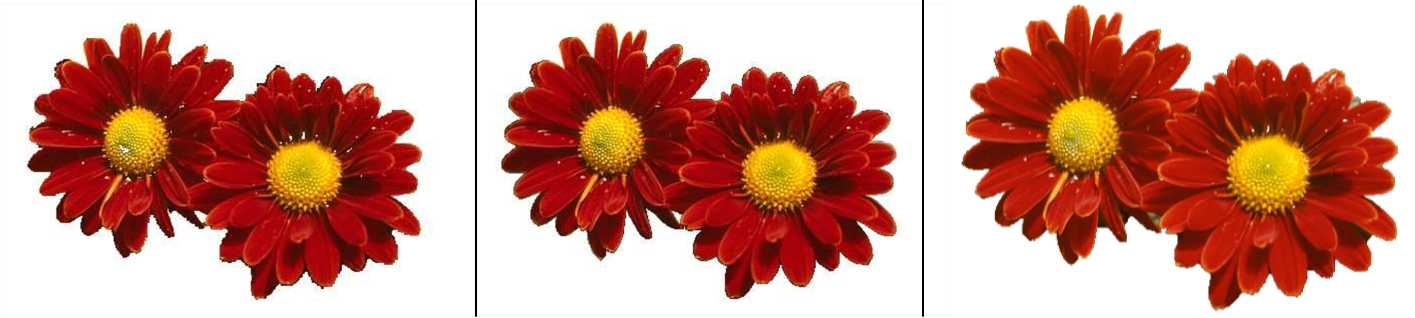
\includegraphics[width=\linewidth]{Experiments/figures/124080.png}
\\
  \caption{\label{fig:flower_results}GrabCut Results.}
  \end{center}
\end{figure}

\begin{figure}[ht]
  \begin{center} \setlength{\tabcolsep}{0pt}
    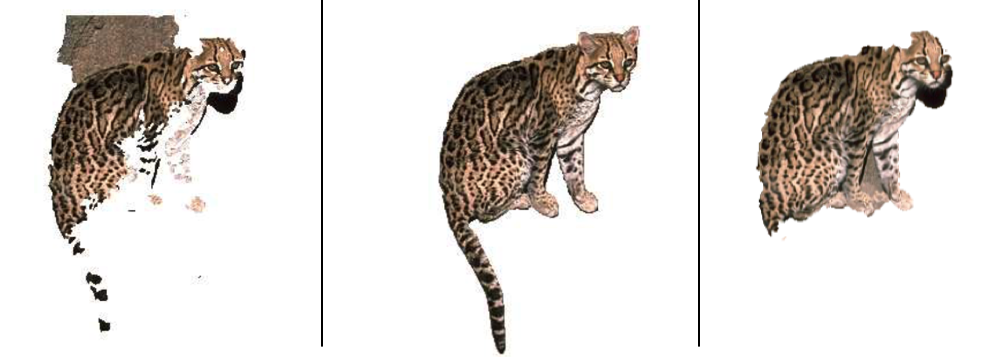
\includegraphics[width=\linewidth]{Experiments/figures/326038.png}
\\
  \caption{\label{fig:cheetah_results}GrabCut Results.}
  \end{center}
\end{figure}

\begin{figure}[ht]
  \begin{center} \setlength{\tabcolsep}{0pt}
    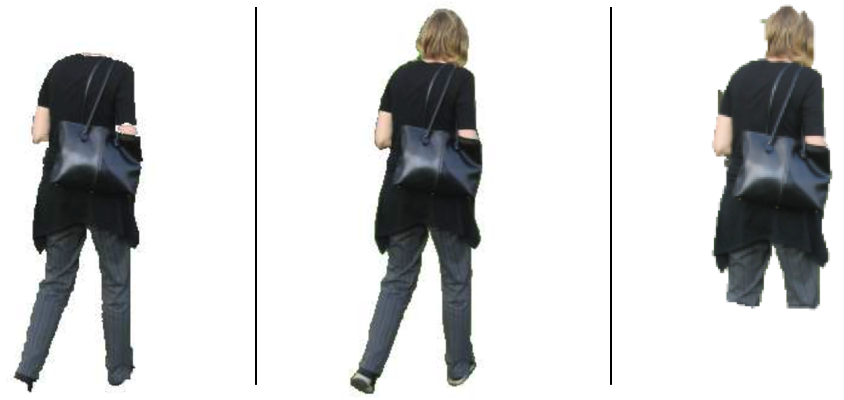
\includegraphics[width=\linewidth]{Experiments/figures/person5.png}\\
  \caption{\label{fig:person_results}GrabCut Results.}
  \end{center}
\end{figure}

In figure~\ref{fig:flower_results}, our new method has a very
strong results. It almost perfectly extracted the foreground
image. The accuracy is over $99.5\%$. In
figure~\ref{fig:cheetah_results} our new method still performs
better. However, it left the cheetah's tail out compared to our
previous method. One important thing to notice is that there are
many holes in the image on the left (inferred by our previous
method) while the image inferred by our new method is very smooth
without holes. This certificates that by learning the lower
linear envelope exactly, our new method has a better performance
on preserving higher order consistency. In
figure~\ref{fig:person_results} two methods have almost the same
performance. Previous method left the woman's head but was
able to capture her full legs while our new method only able to
capture half of her legs but with full head.

\bigskip
\bigskip
\bigskip
\bigskip

However, the performance various significantly between images. In
figure~\ref{fig:portrait_results}, even though the sculpture
inferred by our new method is still very smooth without any hole
on it, our method failed to segment the background out of the
foreground (there are large amount of pixels belong to stairs and
glass). Our model completely fails to learn the image
``189080.png'' which has the worst performance $42.5\%$ (the
\algref{alg:learning} stopped at the maximum number of iterations
which is 10 \emph{outer loops} and 100 \emph{inner loops} for
each \emph{outer loop}). The inferred foreground image is
completely blank as shown in figure~\ref{fig:grabcut_worst}.


\begin{figure}[t]
  \begin{center} \setlength{\tabcolsep}{0pt}
    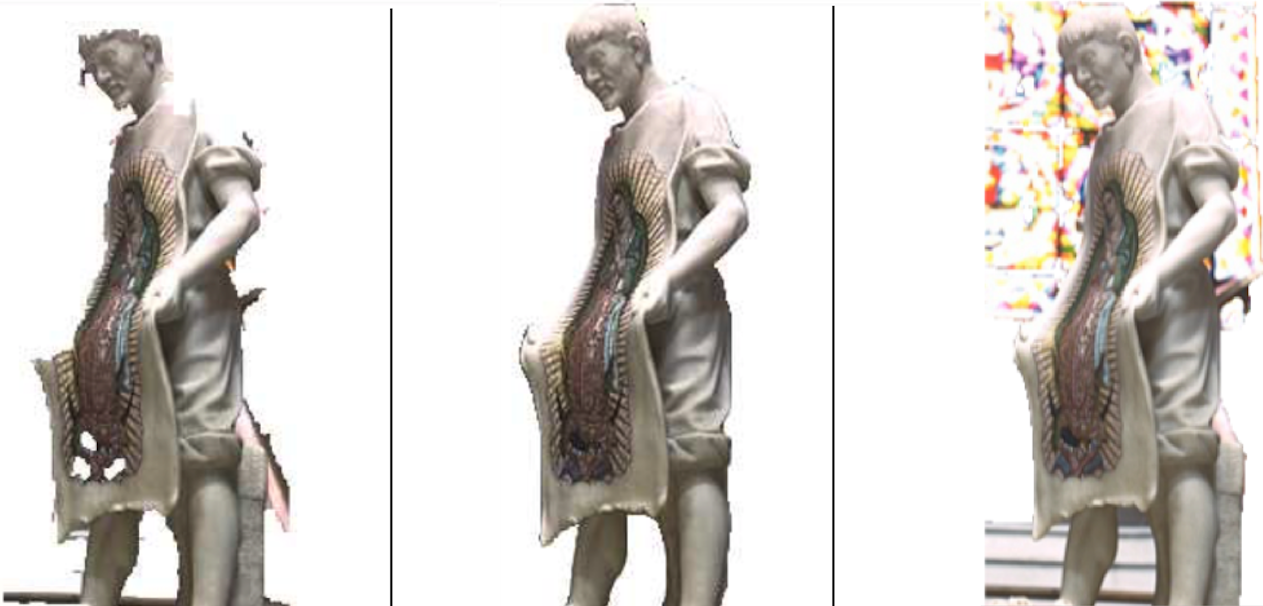
\includegraphics[width=\linewidth]{Experiments/figures/24077.png}\\
  \caption{\label{fig:portrait_results} GrabCut Results.}
  \end{center}
\end{figure}

\begin{figure}[t]
  \begin{center} \setlength{\tabcolsep}{0pt}
    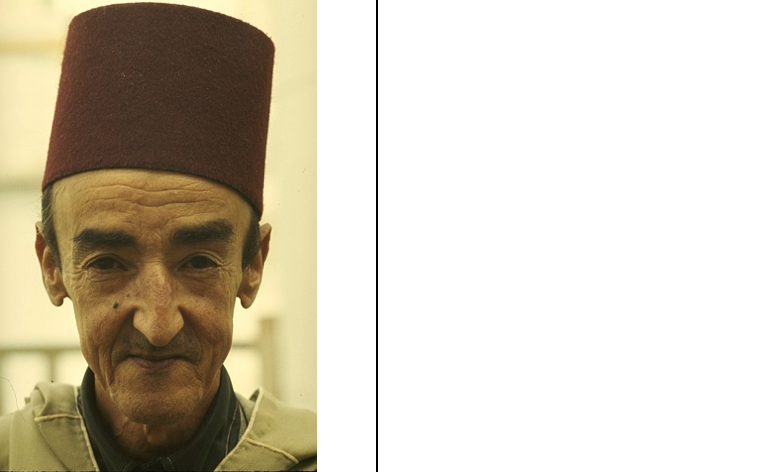
\includegraphics[width=0.5\linewidth]{Experiments/figures/189080.png}
\\
\caption{\label{fig:grabcut_worst} Worst accuracy image. The
  accuracy is only $42.5\%$. The foreground inferred is
  completely blank which means information learned by our model
  is failed to be generalize to this image.}
  \end{center}
\end{figure}

\clearpage

\subsection{Conclusions}
\label{sec:grabcut-conc}

From above experiments we conclude our findings as followings:

\begin{itemize}
\item In general, our new method outperforms previous one.
  The accuracy is increased by $0.6\%$. This might because our
  new method learns the lower linear envelope exactly thus has a
  richer representation than previous one.
\item In general, our new method has a better higher-order
  consistency. This can be seen from
  figure~\ref{fig:flower_results} to
  figure~\ref{fig:portrait_results}. This is also because the
  lower linear envelope function has better quality than our
  previous method.
\item The new method's performance various differently among
  images. The performance ranges from $42.5\%$ to $99.5\%$.
\item The new method is more computationally expensive than our
  previous method during training. It takes $5.3$ hours to train
  one cross-validation fold while previous method only takes
  $3$ hours. However, it is more efficient during testing due to
  it simplicity for the lower linear envelope potentials.
\item There seems like to exist some generalization issues in our
  \algref{alg:learning}. For example, the new method has bad
  performance of filtering background in
  figure~\ref{fig:portrait_results} and it completely fails to
  infer the figure~\ref{fig:grabcut_worst}.
\end{itemize}



\clearpage
\cleardoublepage



%%% Local Variables:
%%% mode: latex
%%% TeX-master: "../thesis"
%%% End:


%% Conclusion
%%
%% Template conclusion.tex
%%

\chapter{Conclusion and Future Work}
\label{cha:conclusion}

We summarize our work in this chapter. We will also conclude its
advantages and disadvantages basing on our synthetic
(section~\ref{sec:synth-check}) and real-world
(section~\ref{sec:foregr-extr}) experiments' results. Our work
also provide some insights to our future work which we will
briefly discuss in this chapter.


\section{Conclusion}
\label{sec:conclusion}

Lower linear envelope binary MRFs are raising interests due to
its capability for encoding higher-order consistency constraints
over large sets of random variables. \citename{gouldlearning} has
shown how to perform exact inference and learning of this problem
under the max margin framework. In order to transform the lower
linear envelope function to a linear combination formulation,
they interpolates it with a set of fixed space sample points.
Thus their algorithm is only able to learn the shape of the lower
linear envelope function approximately.

The main goal of our research is to learn the lower linear
envelope function exactly. Based on their work, we explore a
variant of their formulation by introducing auxiliary variables
back to the energy function to formulate an exact representation.
We find that the lower linear envelope function under the
quadratic pseudo-Boolean formulation~\eqref{eq:originalenergy}
itself is an inner product of parameters and features thus can be
written into a linear combination directly. Under this
formulation the inference algorithm (\emph{st min cut}
construction) developed by \citename{gouldlearning} still adapts
to our problem. Therefore, we are still able to conduct exact
inference on our problem. We developed the learning
\algref{alg:learning} using an extension of the max margin
framework which is known as latent structural SVM. However, this
algorithm is only guaranteed to decrease the objective function
to a local minimum thus the initial point will affect the overall
performance. In order to overcome this issue we also proposed an
empirical initialization \algref{alg:init_theta}.

In order to examine the effectiveness of our new algorithm, we
repeat two experiments \citename{gouldlearning} conducted in
their research and compare both results. In the first synthetic
checkerboard experiment, we found that in general the new
algorithm's accuracy is at least as well as the previous one. But
on harder problem~\ref{sec:unif-distr-squar} the new method
outperforms previous one significantly. The new method is much
more computationally expensive during the training period.
However it is more efficient during the testing stage because of
the simplicity of the shape of the lower linear envelope. We also
found that the shape learned by the new method can shift along
with the changes of the input data which proves that we can learn
the lower linear envelope exactly.

We then take our algorithm to a harder real-world
experiment~\ref{sec:foregr-extr}. It turns out that our new
method has a slightly increasing in overall accuracy (0.6\%)
compared to the previous method. There are much less holes in
images inferred by our new method which certificates the lower
linear envelope function learned by our formulation can better
enforce higher order consistency in large cliques. However, the
performance various significantly between cross-validation folds
which indicates there are some generalization issues existing in
our new method.

At last we summarize the advantages and disadvantages as
following.

\bigskip

Advantages of the new method (compared to the previous
method~\cite{gouldlearning,Gould:ICML2011}):

\begin{itemize}
\item Able to learn the lower linear envelope exactly.
\item Performs better (higher accuracy) on harder problems.
\item Efficient to compute during testing due to the simplicity
  of the shape of the lower linear envelope function.
\end{itemize}

Disadvantages of the new method:

\begin{itemize}
\item Only guaranteed to decrease to the local minimum.
\item Computationally expensive during training.
\item Generalization various significantly.
\end{itemize}




\section{Future Work}
\label{sec:futurework}

As we suggested in the conclusion, our new method seems to have
some generalization issues (figure~\ref{fig:grabcut_worst} for
example). It will be our primal goal to keep investigating into
this problem. We also proposed an empirical initialization method
in section~\ref{sec:mrflssvm_learning_algo}. For future work we
would compare this method to others.

Our research also provide insights to further directions.
Extending our approach to multi-label MRFs seems to be very
promising. Other straightforward extensions include the
introduction of features for modulating the higher-order terms
and the use of dynamic graph cuts~\cite{Kohli:PAMI07} for
accelerating loss-augmented inference within our learning
framework. Other optimization algorithms for solving our learning
problem may also be considered, \eg the subgradient
method~\cite{Nowozin:2011, Bertsekas:2004}.






%%% Local Variables: 
%%% mode: latex
%%% TeX-master: "thesis"
%%% End: 


%%%%%%%%%%%%%%%%%%%%%%%%%%%%%%%%%%%%%%%%%%%%%%%%%%%%%%%%%%%%%%%%%%%%%%
% Here begins the end matter

%%%
%% Template appendix.tex
%%

\appendix

\chapter{Some Other Stuff}
\label{app:app1}

\section{Why I Did It}
\label{sec:why3}

\chapter{More Stuff}
\label{app:app2}

%%% Local Variables: 
%%% mode: latex
%%% TeX-master: "thesis"
%%% End: 


\backmatter

%%%%%%%%%%%%%%%%%%%%%%%%%%%%%%%%%%%%%%%%%%%%%%%%%%%%%%%%%%%%%%%%%%%%%%%
%% Other options
% \end{doublepage}

\bibliographystyle{abbrvnat}
\bibliography{Bibs/thesis,Bibs/long,Bibs/scene}

\printindex

\end{document}

%%% Local Variables: 
%%% mode: latex
%%% TeX-master: "thesis"
%%% End: 



